%  Bachelorarbeit                                           %%
%% TH Köln -Campus Gummersbach, Fak. 10)                    %%
%% 2021                                                     %%
\documentclass[a4paper,12pt,oneside]{article}
% Optionen:
% - a4paper => DIN A4-Format
% - 12pt    => Schriftgröße (weitere  
%              grundlegende Fontgrößen: 10pt, 11pt)
% - oneside => Einseitiger Druck

%% Verwendete Pakete:
\usepackage[ngerman]{babel} % für die deutsche Sprache
\usepackage{caption} % Für schönere Bildunterschriften
\usepackage[T1]{fontenc} % Schriftkodierung (Für Sonderzeichen u.a.)
\usepackage[utf8]{inputenc} % Für die direkte Eingabe von Umlauten im Editor u.a.
\usepackage{fancyhdr} % Für Kopf- und Fußzeilen
\usepackage{lscape} % Für Querformat

%\fancyfoot[RE]{\thepage} % Páginas Pares numeradas a la derecha

%Create Glossar
%\usepackage[xindy,acronym]{glossaries}
%\makeglossaries
%\loadglsentries[chapters]{Glossar.tex}

%% Show code in a better way
\usepackage{listings}
\usepackage{xcolor}

%%Akrnyme
\usepackage{acronym} %[printonlyused]

%% Show code in a better way
\usepackage{listings}
\usepackage{color}

\definecolor{dkgreen}{rgb}{0,0.6,0}
\definecolor{gray}{rgb}{0.5,0.5,0.5}
\definecolor{mauve}{rgb}{0.58,0,0.82}

\lstset{frame=tb,
  language=Java,
  aboveskip=3mm,
  belowskip=3mm,
  showstringspaces=false,
  columns=flexible,
  basicstyle={\small\ttfamily},
  numbers=none,
  numberstyle=\tiny\color{gray},
  keywordstyle=\color{blue},
  commentstyle=\color{dkgreen},
  stringstyle=\color{mauve},
  breaklines=true,
  breakatwhitespace=true,
  tabsize=3
}
%% Schriften (Beispiele)
%% Weitere LaTeX-Schriften im "LaTeX Font Catalogue"
%% unter: http://www.tug.dk/FontCatalogue/.
%% ACHTUNG: Ggf. müssen Schriften noch installiert 
%% werden!

% Serifen-Schriften:
\usepackage{lmodern} % Schriftart "Latin Modern"
%\usepackage{garamond} % Schriftart "Garamond"

%Sans Serif-Schriften:
%\usepackage[scaled]{uarial}
%\usepackage[scaled]{helvet}
%%--------------
\usepackage[normalem]{ulem} % Für das Unterstreichen von Text z.B. mit \uline{}
\usepackage[left=3cm,right=2cm,top=2cm,bottom=2.5cm,
textheight=245mm,textwidth=160mm,includeheadfoot,headsep=1cm,
footskip=1cm,headheight=14.599pt]{geometry} % Einrichtung der Seite 

\usepackage{graphicx} % Zum Laden von Graphiken
\graphicspath{ {./sources/} }

% INFO: Graphiken einbinden
%
% \includegraphics[scale=1.00]{dateiname}
%
% => Ausgabeformat: PDF-Dokument:
%    Es können die folgenden (Graphik-)formate eingebunden
%    werden: .jpg, .png, .pdf, .mps
% 
% => Ausgabeformat: DVI/PS:
%    Folgende (Graphik-)formate werden unterstützt:
%    .eps, .ps, .bmp, .pict, .pntg
\usepackage{epstopdf}

% Pakete für Tabellen
\usepackage{tabularx} % Einfache Tabellen
\usepackage{longtable} % Tabellen als Gleitobjekte (für die Aufteilung bei langen 
 %Tabellen über mehrere Seiten)
\usepackage{multirow} % Für das Verbinden von Zeilen innerhalb einer Tabelle mit
 % \multirow{anzahl}{*}{Text}

% (Zusatz-)Pakete für Formeln
\usepackage{amsmath}
\usepackage{amsthm}
\usepackage{amsfonts}

\usepackage{setspace} % Paket zum Setzen des Zeilenabstandes
% INFO: Zeilenabstand setzen:
%
% Befehle:
% - \singlespacing  => 1-zeilig (Standard)
% - \onehalfspacing => 1,5-zeilig
% - \doublespacing  => 2-zeilig 
\onehalfspacing % Zeilenabstand auf 1,5-zeilig setzen

% Farbboxen (für die Merkkästen in dieser Vorlage):
\usepackage{tcolorbox}
\tcbset{colback=white,colframe=orange,
        fonttitle=\bfseries}

\usepackage[colorlinks,pdfpagelabels,pdfstartview=FitH,
bookmarksopen=true,bookmarksnumbered=true,linkcolor=black,
plainpages=false,hypertexnames=false,citecolor=black, urlcolor=blue]{hyperref} 
% Für Verlinkungen
% INFO: Verlinkungen mit dem hyperref-Paket:
%
% Die Angabe von URLs mit dem Befehl \url{} erlaubt einen
% gesonderten Umgang mit Weblinks. Denn die Links werden verlinkt.
% Auch erfolgt automatisch am Zeilenende ein Umbruch des Links.
% Es ist auch nicht erforderlich, Sonderzeichen in der URL manuell zu 
% entschärfen.
%
% TIPP: Sollte ein Umbuch bei einem Link nicht automatisch erfolgen, so kann
% das daran liegen, dass ein/mehrere Zeichen zusätzlich angegeben werden müssen,
% an dem der Link umbrochen werden kann.
% Dies kann mit folgendem Befehl erfolgen (Beispiel):
% \renewcommand*\UrlBreaks{\do-\do_}

% Das Paket "biblatex" für autom. 
% Literaturverzeichnisse:
%\usepackage{csquotes} % Für sprachangepasste Anführungszeichen
%\usepackage[backend=bibtex,style=ieee]{biblatex}
%\addbibresource{chapters/bibx.bib}           

%This didnt works, because i need  a .bib
%\usepackage[authoryear,round,longnamesfirst]{natbib}

%%%%%%%%%%%%%%%%%%%%%%%%%%%%%%%%%%%%%%%%%%%%%
%% DOKUMENT                                %%
%%%%%%%%%%%%%%%%%%%%%%%%%%%%%%%%%%%%%%%%%%%%%
\begin{document}
% Unbeschriftetes Vorblatt (Leere Seite)
\pagestyle{empty} % Seite ohne Kopf- und Fußzeilen
\newpage % Neue Seite
\input{leereSeite} % Ausgelagerte LaTeX-Datei (hier: leereSeite.tex) einbinden

\newpage
% Deckblatt
\pagestyle{empty}
\begin{titlepage}
  \begin{center}
\includegraphics[scale=0.18]{sources/TH_Koeln_Logo}\\
    \Large
    Technische Hochschule Köln\\
    Fakultät für Informatik und Ingenieurwissenschaften\\
    \hrule\par\rule{0pt}{2cm} % Horizontale Trennlinie  mit 2 cm Abtand nach unten erzeugen
    \LARGE
    \textsc{BACHELORARBEIT}\\
    \vspace{0.8cm} % Vertikaler Abstand von 1cm erzeugen
    \huge
    Kostenüberwachung und -optimierung für Cloud-Dienste am Beispiel von Amazon Web Services \\    
    \vspace{0.8cm}
    \large
    Vorgelegt an der TH Köln Campus Gummersbach\\
    im Studiengang Wirtshaftsinformatik\\
    \vspace{0.8cm}
    ausgearbeitet von:\\
    \textsc{Carlo Menjivar} 11117929\\
    \vspace{0.8cm}
    \begin{tabular}{ll} % Einfache Tabelle ohne Rahmen, mit 2 Spalten erzeugen
      \textbf{Erstprüfer:}  & Prof. Dr. Roman Majewski \\
      \textbf{Zweitprüfer:} & Thomas Raser\\
    \end{tabular}
    \vspace{0.8cm}
    \\Gummersbach, 20 Dezember 2021
  \end{center}
\end{titlepage}
\newpage

\section*{Abstract}\label{kap_Abstract}
\addcontentsline{toc}{section}{Abstract} % Manuellen Eintrag im Inhaltsverzeichnis erzeugen
% Abstract (ACHTUNG: Abweichung zur Reihenfolge im Merkblatt!)
\begin{abstract}
In dieser Arbeit werden Werkzeuge untersucht, die einen klareren Überblick über die finanziellen %und leistungsbezogenen
Ressourcen schaffen[DAS MUSS GEÄNDERT WERDEN]. Mit den gesammelten Informationen dienen sie dazu, direkte Maßnahmen zu ergreifen. Darüber hinaus werden allgemeine Optimierungsmaßnahmen aufgezeigt, die bereits über die Jahre hinweg von anderen Nutzern getestet wurden und von Amazon Web Services (als Best Practices) empfohlen werden.
%die zu erheblichen Kosteneinsparungen in der Cloud führen. 
% Angefangen bei der Wahl des richtigen Zahlungsmodells, über das automatische Herunterfahren ungenutzter Instanzen zu bestimmten Zeiten bis hin zur Implementierung von Autoscaling für EC2-Instanzen.
%WELCHE INFOS BRAUCHEN DIE CLOUD-NUTZER ÜBER DIE kOSTEN; UM DIE RICHTIGE ENTSCHIEDEN ZU TREFFEN.
Die Grundlage dieser Recherche sind Empfehlungen von Cloud-Anbietern bezüglich Kostenüberwachung und -optimierung, Erfahrungen von Experten in dem Fachgebiet und aktuelle Fachliteratur.
\\\\
Es ist besonders interessant für Teams, die Cloud-Dienste in aktuellen Projekten nutzen und ihre Kosten in der Cloud besser verstehen und optimieren wollen. Wenn die Kosten für Cloud-Dienste wie alle anderen Kosten betrachtet werden, ist es konsequent, über ihre Kontrolle und Optimierung nachzudenken. Ein häufiges Problem ist, dass Kosten entstehen, die sich der Kontrolle der Nutzer entziehen.%[ZITAT?]
Aus diesem Grund stehen Unternehmen die bereits On-Premise IT-Infrastruktur nutzen, einem Wechsel kritisch gegenüber, obwohl ihnen die Flexibilität von Cloud-Diensten bessere Wettbewerbsvorteile bieten würde.
Deshalb sind die in dieser Arbeit aufgezeigten Werkzeuge und Maßnahmen relevant für diejenigen, die von einem  Wechsel von klassischen Modellen, bekannt als On-Premise, zu Cloud basierten Modellen profitieren möchten.
\end{abstract}
\newpage
\renewcommand{\abstractname}{Abstract}
\begin{abstract}
    Platz für das englische Abstract....
\end{abstract}


\newpage

% Inhaltsverzeichnis
\tableofcontents
\newpage
\pagestyle{fancy} % Kopf- und Fußzeilen aktivieren (=> Paket "fancyhdr")

% Abbildungsverzeichnis  
% INFO: Abbildung einbinden (Beispiel):
%  \begin{figure}[h!]
%    \centering
%    \includegraphics[scale=1.00]{Pfad zum Bild}\\
%    \caption{Bildunterschrift} 
%    \label{Marke zum Referenzieren auf die Abbildung}
%  \end{figure}


\section*{Abbildungsverzeichnis}
\addcontentsline{toc}{section}{Abbildungsverzeichnis} % Manuellen Eintrag im Inhaltsverzeichnis erzeugen
\renewcommand{\listfigurename}{} % Name des Abbildungsverzeichnisses ändern
\thispagestyle{empty}
\listoffigures
\newpage

%Temporär, danach sollten wir das Package glossaries benutzen
\section*{Glossar}\label{kap_glossar}
\addcontentsline{toc}{section}{Glossar} % Manuellen Eintrag im Inhaltsverzeichnis erzeugen
%\newglossaryentry{kiln}
%{
 % name=kiln,
  %description={German: Brennofen (m.);\\Français: fourneau (m.)},
  %plural=kilns
%}

%Make Glossary properly...
%\acrodef{VB}{Visula Basic}

\textbf{Cloud-Computing:}\\
...
\\\\
\textbf{Cloud-Dienste:}\\
...
\\\\
\textbf{On-Demand:}\\
...
\\\\
\textbf{On-Premise:}\\
...
\\\\
\textbf{Region:}\\
Die Region ist ein völlig unabhängiges und eigenständiges geografisches Gebiet. Jede Region hat mehrere, physisch getrennte und isolierte Standorte, die als Availability Zones bekannt sind. Beispiele für Regionen sind London, Dublin, Sydney, usw \footnote{\cite{AWS1}, Seite 42}.
\\\\
\textbf{Availability Zone:}\\
Eine Verfügbarkeitszone ist einfach ein Datenzentrum oder eine Sammlung von Datenzentren. Jede Verfügbarkeitszone in einer Region verfügt über eine separate Stromversorgung, Netzwerk und Konnektivität, um die Gefahr eines gleichzeitigen Ausfalls in beiden Zonen zu verringern \footnote{\cite{AWS1}, Seite 42}.
\\\\

\textbf{Instance family:}\\
Instanzfamilien sind eine Sammlung von EC2-Instanzen, die nach dem Verhältnis von Speicher, Netzwerkleistung, CPU-Größe und Speicherwerten zueinander gruppiert sind. Zum Beispiel bietet die m4-Familie von EC2 eine ausbalancierte Kombination von Rechen-, Speicher- und Netzwerkressourcen. \footnote{\cite{AWS1}, Seite 95}.
\\\\
Instagram-Story
\\\\
Tag
\\\\
Buckets
\\\\
PAYG %https://www.nimbix.net/glossary/pay-go
\\\\
Metadaten
\\\\
Startkonfiguration %https://docs.aws.amazon.com/autoscaling/ec2/userguide/create-launch-template.html
\\\\
Scale-In/Out
%\\\\
%Governance, Compliance ?
%\\\\
\newpage

\section*{Abkürzungsverzeichnis}\label{kap_Abkuerzungen}
\addcontentsline{toc}{section}{Abkürzungsverzeichnis} % Manuellen Eintrag im Inhaltsverzeichnis erzeugen
\input{chapters/Abkürzungsverzeichnis}
\newpage

\section{Einleitung}\label{kap_einleitung}
%\addcontentsline{toc}{section}{Einleitung} % Manuellen Eintrag im Inhaltsverzeichnis erzeugen
%Motivation und Ziele als subsecion?
%WEITERE QUELLE Für mOTIVATION
%https://www.gartner.com/smarterwithgartner/4-trends-impacting-cloud-adoption-in-2020
%\subsection*{Einführung in das Thema (Motivation, zentrale Begriffe etc.)}
\subsection{Motivation}
%\addcontentsline{toc}{subsection}{Motivation}
%WARUM HABE ICH MICH FÜR AWS ENTSCHIEDEN?
%Wie viele Firmen wechseln von On-Premise zu Cloud in DE jährlich?
[Persönliches Statement... wieso schreib ich das hier eigentlich ;)] Die zunehmende Digitalisierung von Geschäftsmodellen, die auch durch die Corona-Pandemie vorangetrieben wird, lässt Cloud-basierte Applikationen an Bedeutung gewinnen.\footnote{Es sei an diser Stelle darauf hingewiesen, dass in diesem Kontext Ahrens die Bedeutung Cloud-basierter Anwendungen im Bereich von deutschen Handelsunternehmen untersuchte (Vgl. Ahrens 2021)\cite{STA3}, sowie das \textit{ifo Institut} anschaulich die strukturellen Veränderungen von der Corona-Pandemie auf den Arbeitsalltag in Deutschland nachzeichnete (Vgl. ifo Institut 2020)\cite{STA2}.} Als direkte Folge davon ist die Nachfrage nach Server- und Speicherkapazität gestiegen.
%Dies wird auch von 48\% der befragten Handelsunternehmen im Jahr 2021 bestätigt.
Die Relevanz von \textit{Amazon Web Services}, kurz AWS, in dem Bereich der Cloud-Computing ergibt sich aus einer vor kurzem veröffentlichte Studie von Raj Bala et al.. Diese wies eindrücklich daraufhin, dass AWS der aktuell weltweit führende Cloud-Anbieter anhand ihrer Klassifikation (\textit{Magic Quadrant}\footnote{ Laut Gartner stellt der Magic Quadrant eine zweidimensionale Matrix mit vier Quadranten dar. Jeder Quadrant steht für einen Unternehmenstypus im Markt. Im Uhrzeigersinn von links unten beginnend sind dies: \textit{Nichenanbieter, Herausforderer, Marktführer }und \textit{Visionäre}}) für Cloud-Infrastruktur und Plattform-Services sei (Bala et al, 2021, o.S.,\cite{G01}).
AWS erscheint nicht nur aus diesem Grund als Fallbeispiel für diese Arbeit passend, weitere bedeutsame Faktoren sind seine frühe Präsenz (2006) als Cloudanbieter und seines großen Angebotes an Cloud-Diensten, welche für zahlreiche Anwendungsfälle geeignet sind.\footnote{ Die aktuellen Marktführer im Bereich der \textit{Cloud-Computing} weltweit sind AWS, Google, Telekom und Microsoft (Vgl. Synergy Reseach Group 2019, o.S.\cite{STA6})}
\\\\

\begin{comment} GELÖSCHT, WEIL DIESE EINE BEHAUPTUNG IST (25.10.2021)
    \\\\
    Für viele Unternehmen ist eine große Herausforderung, die Kosten von Cloud-Diensten übersichtlich zu halten und Optimierungsmöglichkeit leicht zu erkennen. Zusätzlich besteht die Gefahr, unangenehme Überraschungen in einer Rechnung zu bekommen, weil keine Grenze für den Konsum von Cloud-Diensten festgelegt wurde. 
    \end{comment}
\subsection{Problemstellung}
%\addcontentsline{toc}{subsection}{Problemstellung}
%Wenn ein Hotel die Vorteile von dem Cloud-Computing hätte, dann könnte dieses folgendermaßen funktionieren:
\begin{comment}
\\\\
”Heute hatten wir 17 Gäste für unsere derzeit 20 Zimmer. Für die kommende Messe am Wochenende sind wir bereit 500 Gäste zu empfangen. Nach der Messe werden wir mit unseren üblichen 20 Zimmern wie immer gut arbeiten können.”
Normalerweise bräuchte man eine große Investition zu machen, um solche kurzfristige Nachfrage zu erfüllen. Vergleichbar ist es bei traditionellen IT-Infrastrukturen, mehr Kapazitätsbedarf, würde die Anschaffung von einer neuen Hardware bedeuten.
\\\\
\end{comment}
%Die Verwendung von Cloud-Diensten bringt viele Vorteile mit sich. Zum Beispiel kurzfristige Erhöhung oder Verringerung der Speicher- und Rechenkapazität, sowie Zugriff auf unterschiedliche Speicherarten, die genau an individuelle Anwendungsfälle angepasst sind. All diese Lösungen sind in wenigen Minuten einsatzfertig. 
%\\\\
%Viele Unternehmen befürchten jedoch, dass der Wechsel von On-Premise zu On-Demand zu hohen Kosten führen könnte.
%In einer Umfrage haben circa 50\% der Unternehmen die Verwaltung der Kosten für den Betrieb von Cloud-Workloads als großes Hindernis genannt. Mehr als die Hälfte der Befragten haben geäußert, dass sie Schwierigkeiten haben, alle Kosten für Cloud-Workloads zu rechtfertigen.
Adam Stern wies in dem \textit{Forbes}-Magazin daraufhin, dass ungefähr die Hälfte der US-amerikanischen Unternehmen Schwierigkeiten hätten ihre Kosten zu begründen (Stern 2018, o.S.). 
\begin{quote}
    „In its Stratecast Predictions 2018, Frost \& Sullivan noted that 53\% of IT leaders surveyed cited “managing costs to run cloud workloads” as a huge obstacle, and over 50\% have difficulty justifying the expenses of some public cloud workloads.“  
    \footnote{Stern, Adam, The Truth About Cloud Pricing.\cite{SP1}}
\end{quote}
Darüber hinaus weist Tobias Regenfuß und Jochen Malinowski
von Accenture GmbH in einer Untersuchung, dass es den Unternehmen an fachlichem Know-How in Cloud-Computing mangelte. Diese stelle eine der größten Hindernisse dar, um einen Wechsel von On-Premise- zu Cloud-basierten Systemen gewährleisten zu können\footnote{Regenfuß und MalinowskiStern, Hohe Erwartungen an die Cloud: Hürden meistern, Mehrwert maximieren. 2020 o.S.(Webversion) oder S.11 in der PDF-Version auf Englisch\cite{ACC1}}.
\\\\
Kostenoptimierung für Cloud-Dienste ist ein wichtiger Punkt, da man ohne Optimierungsmaßnahmen mit höheren Kosten rechnen müsse als bei On-Premise Systemen(Anders Lisdorf\footnote{Anders Lisdorf. Cloud Computing Basics: a Non.-Technical Introduction. S.152. \cite{CCB}}).
\\
([Rev] SOLLTE DIE UNTERE DIREKTE ZITAT WEG)
\begin{quote}
    ”Indeed, if you run the cloud the same way you run your on-premise data center, you are almost certain to incur higher expenses. It is necessary to use the following key cloud cost optimization techniques in order to successfully save money on the cloud.”
    \footnote{Anders Lisdorf. Cloud Computing Basics: a Non.-Technical Introduction. S.152. \cite{CCB}}
\end{quote}
\begin{flushleft}
Diese Bachelorarbeit beschäftigt sich mit ebendieser Problematik, um herauszufinden, wie Unternehmen mit den passenden Werkzeugen die Kosten ihrer Cloud-Dienste überwachen und im Blick behalten können. %Zum Beispiel können frühzeitige Benachrichtigungen alarmieren, wenn Cloud-Dienste mehr Kosten verursachen als geplant.
\\
Außerdem sollte untersucht werden, wie mit der richtigen Auswahl an Diensten Kosten optimiert werden. 
%In dieser Arbeit wird versucht zu beantworten, wie Kosten bei Cloud-Diensten überwacht werden können. Auf Grundlage dieser Information werden Optimierungsmöglichkeiten untersucht. 
Es wird untersucht, welche Maßnahmen nötig sind, um unerwartet hohe Kosten bei Cloud-Diensten zu vermeiden. Darüber hinaus werden Empfehlungen von Cloud-Experten berücksichtigt, um Kosten von Cloud-Diensten zu minimieren. Diese Arbeit untersucht speziell die Kostenoptimierung  von S3-Speichereinheiten und EC2-Server-Instanzen mithilfe von folgenden Überwachungswerkzeuge: Cost-Explorer, CloudWatch und Trusted Advisor.
\end{flushleft}


\subsection{Zielsetzung}
%\addcontentsline{toc}{subsection}{Zielsetzung}
Die vorliegende Arbeit betrachtet die von AWS angebotenen Überwachungswerkzeuge, um ein tiefergehendes Verständnis der Entstehung von Kosten durch die Nutzung von Cloud-Diensten zu gewährleisten. Mit den von AWS zur Verfügung gestellten Maßnahmen sollen die Nutzung und damit die Kosten von Cloud-Diensten reduziert werden.
%\textbf{Daraus ergeben sich für die Arbeit die folgenden Ziele:}%\\ 
%\%begin{itemize}
 %   \item
 %       Als Erstes wird gezeigt, wie mithilfe von bestehenden %Werkzeugen  die Kosten von Cloud-Diensten überwacht %werden können.
  %  \item
 %       Als Nächstes wird anhand von Empfehlungen von Cloud-Experten identifiziert, welche Optimierungsmöglichkeiten bestehen.\\
%\end{itemize}

%Die vorgestellten Werkzeuge werden auf eine Testumgebung eingesetzt und deren Auswirkungen im Bezug auf die Kosten %bewertet.\\
\begin{comment}
\subsection*{Einschränkungen}
\addcontentsline{toc}{subsection}{Einschränkungen}

Der Schwerpunkt dieser Arbeit liegt auf EC2-Instanzen, da diese in der Regel den größten Anteil an der Rechnung ausmachen.
An zweiter Stelle stehen S3-Speichereinheiten, weil sie einen erheblichen Teil der Kosten darstellen.
%STATISTEN DIE DAS BELEGEN?

%Nach Angaben von Amazon Web Services ist es möglich bis zu 90% für EC2 zu sparen, wenn EC2 Spot-Instanzen benutzt werden. 
%Eine Preisreduzierung für Speichereinheiten ist möglich, wenn die richtige Speicherart ausgewählt wird. 
{\cite{AMZ08,AMZ09}} 
\\
Diese Arbeit legt den Fokus auf die Optimierung der oben genannten Dienste.
Als Überwachungswerkzeuge für die Kosten werden die AWS CloudWatch, der AWS Cost-Explorer und der AWS Trusted Advisor untersucht. 
\end{comment}
\subsection{Struktur der Arbeit}
%\addcontentsline{toc}{subsection}{Struktur der Arbeit}

%Schlüsselbegriffe
%Zunächst wird es eine kurze Einführung in die relevanten Begriffe geben, die für die zu untersuchenden AWS-Cloud-Services wichtig sind.

Diese Bachelorarbeit ist in folgende Kapitel unterteilt:\\\\
%2 Die gängigsten Cloud-Dienste, bei deren Geld verschwendet wird.
\textbf{Kapitel~\ref{kap_grundlagen}} 
befasst sich mit dem Begriff Cloud-Economy und erläutert das Potenzial der Cloud-Diensten im wirtschaftlichen Sinne. Die Cloud-Dienste EC2-Instanzen und S3 Speichereinheiten werden ebenfalls kurz erklärt. %Diese dienen als Grundlage für diese Arbeit. 
\\\\
%4 Überwachung von Kosten
\textbf{Kapitel~\ref{kap_zahlungsmodelle}} 
zeigt die verschiedenen Zahlungsmodelle für EC2-Instanzen. Es werden Kriterien vorgestellt, die helfen sollen, sich für das richtige Zahlungsmodell bei verschiedenen Szenarien zu entscheiden. 
\\\\
%5 AWS Cost Explorer und AWS-Kosten- und Nutzungsbericht
\textbf{In Kapitel~\ref{kap_kostenüberwachung }} werden die Werkzeuge eingeführt, die zur Überwachung der Kosten von Cloud-Diensten eingesetzt werden.
\\\\
%4 Methoden zur Kostenbremse
%4.1 S3 Intelligent-Tiering
%4.2 Instance-Scheduler für EC2 und AWS Reserved-Instance
\textbf{Kapitel~\ref{kap_Optimierung}} befasst sich mit Optimierungsmaßnahmen %insbesondere 
für EC2-Instanzen und S3 Speichereinheiten.

%Testumgebung
%Schließlich werden anhand eines Fallbeispiels in \textbf{Kapitel 5?}, die oben genannten Werkzeuge und Techniken in einer %kostenlosen Testumgebung getestet. Um die Zuverlässigkeit der Ergebnisse zu gewährleisten, wird alles gemacht, um die %Vorher- und Nachher-Szenarien vergleichbar zu machen. Dabei werden die Anzahl der Instanzen und deren Auslastung sowie %die Daten auf den Speichereinheiten berücksichtigt.
 

\newpage

%Eizelne Kapitel mit Nummerierung
\section{Grundlagen}\label{kap_grundlagen}
In diesem Grundlagenkapitel werden Erfolgschancen für Unternehmen aufgelistet, die Cloud-Dienste in ihre Geschäftsprozesse integrieren. Mit Cloud-Diensten sind die Dienste eines beliebigen Cloud-Anbieters im Allgemeinen gemeint und nicht ausschließlich AWS-Dienste. 
Es wird ebenfalls erklärt warum Kostenoptimierung und -überwachung relevant für Unternehmen sind.
\\\\
Folgende Ergebnisse könnten durch die Einführung von Überwachungs- und Optimierungsmaßnahmen erreicht werden:
\begin{itemize}
      \item
            Die Möglichkeit, die Kosten verschiedener Projekte, die über dieselbe Infrastruktur laufen, zu trennen.
            Auf diese Weise kann zwischen Projekten, die mehr, und Projekten, die weniger Kosten verursachen unterschieden werden.%Davor Kunden und nicht Projekte
      \item
            Eine beachtliche Erhöhung der finanziellen Rentabilität im Unternehmen.%[ZITAT].
      \item
            Eine geringere Ungewissheit bei der Umsetzung von cloudbasierten Systemen.
      \item
            Mehr Kontrolle über die Gesamtkosten des Betriebs, den sogenannten \textit{TCO}.\footnote{TCO steht für \textit{Total Cost of Ownership}(Vgl. Gartner, o.J., o.S.\cite{TCO}.)}{ }\footnote{Vgl. Ubuntu, delivered by Canonical: A business guide to hybrid/multi-cloud, S.2.\cite{CAN01}}

\end{itemize}
%Basandose en "Vor- und Nachteile der Nutzung von Cloud-Diensten (mit mobilen Endgeräten) in Organisationen und deren Einfluss auf die Nachhaltigkeit"
% Debería aclarar los aspectos principales de mi BA
% En mi caso: 

%1-Cuales son los miedos, razones y oportunidades para las empresas en la NUBE?

%\subsection{Risiken und Oportunitäten der Cloud...}\label{subsec_UabsGrund2}
%Vor- und Nachteile / ?

\subsection{Cloud Economics}\label{subsec_UabsGrund3}
%Was bietet die Cloud den Unternehmen?
%Economics of Cloud Computing
%https://d1.awsstatic.com/whitepapers/introduction-to-aws-cloud-economics-final.pdf
%[Date last review: 25.11 Isa]
%\begin{flushleft}
%\textit{On-Demand Prinzip} kann zum Beispiel die Rechenkapazität je nach Bedarf angepasst werden 
\textit{Cloud Economics} befasst sich mit den Kosten und den Vorteilen von Cloud Computing und die dahinterstehenden wirtschaftlichen Grundsätzen. Anhand des \textit{Pay-as-you-go-Modell (PAYG)} können zum Beispiel nur die Cloud-Dienste in Anspruch genommen werden, die in dem Moment für das Unternehmen gebraucht werden. Damit entfällt die Notwendigkeit hohe Investitionen in Hardware zu tätigen, wie bei On-Premise-Systemen, wo Hardware im Voraus für den künftigen Bedarf.\footnote{Vgl. Anders Lisdorf, 2021, Cloud Computing Basics: a Non.-Technical Introduction, S.23\cite{CCB}} Durch den Verzicht auf Hardware entfallen die Kosten für Reparatur und Wartung. Die Cloud-Anbieter übernehmen dabei viele Verwaltungsaufgaben. Laut Larry Carvalho und Matthew Marden führe dies zu einer Abnahme der nötigen Fachkräften.\footnote{Larry Carvalho and Matthew Marden, 2015, Quantifying the Business Value of Amazon Web Services, S.1\cite{IDC01}} So ist die die Nutzung von Cloud-Diensten in unabhängiger Weise möglich; in Selbstbedienung und mit der Freiheit Dienste ohne Einschränkungen zu gebrauchen. Das bedeutet jedoch gleichzeitig, dass die Nutzerin oder der Nutzer von Cloud-Diensten Verantwortung für die anfallenden Kosten übernehmen.
%\end{flushleft}
%[Grafik der Kosten On-Premise/Demand?]

\subsubsection{Skalierbarkeit}
Hierbei bezieht sich diese Arbeit auf die Möglichkeit, die Kapazität von Cloud-Diensten zu skalieren. Um die Leistung der IT-Infrastruktur aufrecht zu halten, ist es zum Beispiel möglich, das Serversystem so zu konfigurieren, dass es auf wechselnde Lastanforderungen reagiert.
%bietet  ist es möglich die Rechenkapazität hoch- und runterzuskalieren.
%Vertikal und Horizontal
%
%DOPPELT?Mit Auto Scaling wird sichergestellt, dass die Rechenkapazität in Zeiträumen von hoher Nachfrage automatisch hochskaliert.[AUCH RUNTER?]
% davor:  Anzahl der Amazon Server-Instanzen ABER ANZAHL VON SERVERN != Rechenkap.
% und damit Kosten minimieren.
Auf diese Weise kann Zeit mit der Verwaltung von IT-Infrastruktur eingespart werden, welche dann genutzt werden kann, um sich auf die wesentlichen Geschäftsaktivitäten zu konzentrieren.
\footnote{Mark Wilkins, 2021, AWS Certified Solutions Architect - Associate (SAA-C02), S.29.\cite{AWS1}}
%\parencite[][Seite 29]{AWS1} 
%\footnote{Vgl. [p.~29]\cite{AWS1}[]}
%OPTION 2: 
%Auf diese Weise wird Zeit mit der Verwaltung von IT-Ressourcen gespart und es kann sich auf die wesentlichen Geschäftsaktivitäten konzentrieren.
% Davor: 
%Auf diese Weise kann weniger Zeit mit der Verwaltung von IT-Ressourcen verbracht werden und sich mehr auf wesentliche Geschäftsaktivitäten konzentriert werden\footnote{Vgl. {\cite{AWS1}}, Seite 29}.
%\\\\
Dies war der Fall bei \textit{Walgreens} im Jahre 2020 in den Vereinigten Staaten.
Sie haben unter anderem 750 virtuelle Maschinen und \textit{SAP HANA} auf \textit{Azure Instanzen} migriert.
Diesbezüglich kommentierte Dan Regalado:
\begin{quote}
      By getting out of the business of managing datacenters, WBA[Walgreens Boots Alliance] can spend less time worrying about managing IT resources and more time focusing on what it’s really good at—delivering great healthcare and retail experiences to its customers. Azure also gives WBA an opportunity to better utilize the capabilities of its SAP implementation. “One of the key reasons for moving to Azure was so that we could take advantage of the scalability that SAP HANA is capable of,” explains Regalado. “Instead of using extremely big SAP HANA Large Instances, we can start using smaller VMs[virtuelle Maschinen] and then scale out.\footnote{Microsoft, 2020, Customer Story-Walgreens Boots Alliance delivers superior customer service with SAP solutions on Azure, o.S. \cite{AZU01}}
\end{quote}
So erklärte Dan Regalado, dass \textit{Walgreens} mit dem Einsatz von kleinen Instanzen und Auto-Scaling eine Serverinfrastruktur erreicht hat, die sich dem Bedarf an Rechenkapazität anpasst. 

\subsubsection{Flexibilität}% und Agilität}
Hiermit ist die Möglichkeit gemeint, wenn nötig und unter den Bedingungen des Cloud-Anbieters, Cloud-Dienste in Auftrag zu geben und kündigen. Für Cloud-Dienste gibt es im Allgemeinen eine Vielzahl von Optionen, von denen einige Beispiele unten aufgeführt werden:
\begin{itemize}
\item
    Verschiedene Betriebssysteme, ohne oder mit Lizenzierung.
\item
    Die meistverbreiteten Programmiersprachen, unter anderem \textit{Java, C++, Go, JavaScript und Python}.{\cite{AMZ03}}
\item
    Hosting für statische Webseiten und Webanwendungen{\cite{AMZ04}}.
\item
    Populäre relationale und nicht relationale Datenbanken{\cite{AMZ10}}.           
\item
    Vielfältige Hardware-Konfigurationen.

\end{itemize}
Durch die Vielzahl der verfügbaren Diensten ist es möglich, Prototypen und Experimente in kurzer Zeit durchzuführen.\footnote{Vgl. IDC, 2015, Business Value of AWS S.7\cite{IDC01}} Softwareprojekte können schnell auf den Markt gebracht werden. Je nach ihrem Erfolg ist es möglich, sinnvolle und kosteneffizientere Entscheidungen zu treffen. Wenn ein Projekt, aus welchen Gründen auch immer, kurzfristig eingestellt werden muss, könnten alle damit verbundenen Kosten ausfallen. Denn im Gegensatz zu On-Premise-Infrastrukturen gibt es keine Bindung an kostspielige Hardware.
%Wenn die Neuentwicklung nicht erfolgreich war, müssen keine weitere Kosten anfallen.
%Da die verwendete Dienste vollständig stillgelegt werden können.

\subsubsection{Selbstbedienung}
Mit geringem Aufwand ist es möglich, Cloud-Dienste eigenständig einzurichten. Dies hat den Vorteil, dass keine weiteren Personen, wie externe Spezialisten oder die Vertriebsabteilung des Cloud-Anbieters  benötigt werden.\footnote{Vgl. Anders Lisdorf, 2021, Cloud Computing Basics: a Non.-Technical Introduction, S.28\cite{CCB}}
Andererseits besteht ebenso die Gefahr, dass hohe ungewollte Kosten entstehen, wenn jemand versehentlich oder in unverantwortlicher Weise Dienstleistungen in Anspruch nimmt.    
%[TODO: ADD USE CASE WHERE THIS HAPPEND]
%LinkedIn Learning, the woman said something like that?
%BRINGT DIESE UNTERKAP. ETWAS ZUR ARBEIT BEI?

\subsubsection{Keine Vorabkosten}
%https://aws.amazon.com/de/ec2/pricing/
Das Pay-as-you-go-Modell (PAYG) wird von einer Reihe von Cloud-Anbietern angeboten.\footnote{Die aktuellen Marktführer im Bereich der \textit{Cloud-Computing} weltweit sind AWS, Google, Telekom und Microsoft (Vgl. Synergy Reseach Group 2019, o.S.\cite{STA6}).} Dieses erfordert keine Vorauszahlungen für die Nutzung den verschiedenen Cloud-Diensten. Wenn nur für die monatlich verbrauchten Diensten bezahlt wird, verringert sich zudem die Anfangsinvestition in die IT-Infrastruktur oder fällt ganz weg. Dies ist besonders für kleine Unternehmen bedeutsam, die nicht über die finanziellen Mittel verfügen, um in eine IT-Infrastruktur zu investieren. Es besteht jedoch die Möglichkeit, bestimmte Beträge für die zu konsumierende Dienste im Voraus zu bezahlen.\footnote{Im Unterkapitel \ref{sssec:Vorauszahlung} wird eine Berechnung der Einsparungen durch die teilweise oder vollständige Vorauszahlung der Kosten für die Nutzung von Serverinstanzen gezeigt.}  

%\subsubsection{Verfügbarkeit?} t.ly/bV1z
\subsubsection{Technische Fachkompetenz}
Bei einem Einsatz von Cloud-Diensten ist zu bedenken, dass weitere Investitionen wie technische Schulungen für das Personal erforderlich werden. Der \textit{TÜV Rheinland} bietet zum Beispiel Kurse zur Ausbildung von \textit{Cloud Architekten} an. Die Kurse dauern i.d.R. drei Tage und kosten 2.136,05 € pro Teilnehmer. Maßnahmen wie die genannten Kurse wirken so einem der Hauptprobleme entgegen, mit denen Unternehmen bei der Migration in die Cloud konfrontiert werden. Regenfuß und Malinowski stellten heraus, dass in einer von \textit{Accenture} im Jahr 2020 durchgeführten Umfrage 38\% der Befragten angaben, dass fehlende Kompetenzen im Unternehmen in Bezug auf die Cloud ein Hindernis für eine Cloud-Migration seien.\footnote{Regenfuß und Malinowski (Accenture), 2020, Hohe Erwartungen an die Cloud: Hürden meistern, Mehrwert maximieren, S.11\cite{ACC1}}
%[KOSTEN EINER IT-INFRA = SERVER+Rack]
% QUE PORTENTAJE DE LA INVERSION REPRESENTA LA INFRAESTRUCTURA DE IT EN UNA START UP Y EN UNA CORPORACION? RAZONES USAR LA NUBE(Statista)?

\subsection{Amazon Cloud-Dienste}%Sarah 6.12
Im Folgenden liegt der Fokus auf \textit{AWS-Diensten}. Einer der am häufigsten genutzten AWS-Dienste ist \textit{Amazon Elastic Computing Instances EC2}, mit dem virtuelle Maschinen erstellt werden können.\footnote{Kimberly Mlitz, 2021, Cloud infrastructure services vendor market share worldwide from 4th quarter 2017 to 3rd quarter 2021, o.S.\cite{STA4}} Ein weiterer wichtiger AWS-Dienst ist \textit{Amazon Simple Storage Service (S3)}, der zum Speichern von Objekten verwendet wird.\footnote{Objekte sind in AWS die Grundeinheit in welchen Dateien in den Amazon S3-Speichereinheiten gespeichert werden. Neben den Objekten werden Metadaten, wie das Datum der Objekterstellung und das Datum der letzten Aktualisierung gespeichert.(Vgl. Amazon Simple Storage Service User Guide, S.4\cite{AMZ18})}{ }\footnote{Amazon Elastic Computing Instances EC2 werden im Folgenden als \textit{EC2-Instanzen} und Amazon Simple Storage Service als \textit{Amazon S3} oder \textit{Amazon S3-Speichereinheiten} bezeichnet.}
\\\\
Wie Lynn Langit, eine erfahrene Cloud-Architektin, feststellte, könne bis zu 80\% der AWS-Rechnung aus Gebühren für EC2-Instanzen bestehen.\footnote{Lynn Langit, 2021, LinkedIn Learning: AWS Controlling Cost. Minute 0:20-0:45\cite{LINK2}} Laut des \textit{AWS Solutions Architekten} Daniel Peña Silva ist Amazon S3 einer der am häufigsten genutzten AWS-Dienste.\footnote{Vgl. Daniel Peña Silva, 2021, LinkedIn: Listado de todos los Servicios de AWS.\cite{LINK1}} Deshalb fokussiert sich diese Arbeit auf die Überwachungs- und Optimierungsmaßnahmen, hauptsächlich für EC2-Instanzen und Amazon S3.  %\subsubsection*{Amazon Elastic Computing Instances EC2}
%, Sektion 2 Control Costs by Service, Video AWS service type Minute 00:30}.%\subsubsection*{Amazon Simple Storage Service S3} Warum S3 t.ly/iWn3
%S3 ist der Speicherdienst für Objekte bei AWS. 
%der Rangliste vieler Informatikwebseiten und 
%BESSER: S3 WIRD IN BÜCHER WIE t.ly/IJc1 GENANNT? THIS IS A SPANISH CITAT!
\\\\
Wie aus der \autoref{fig:moreCloudStorageThanLocal} hervorgeht ist, werden darüber hinaus seit 2020 weltweit mehr Daten in Serverfarmen als auf lokalen Geräten gespeichert.\footnote{Vgl. Statista: 2020 überholt die Cloud lokale Speichermedien.\cite{STA1}} Dies bietet einerseits  Vorteile im Bezug auf die Geschwindigkeit der Arbeitsabläufe, andererseits birgt aber auch Risiken wie Datendiebstahl. Das Thema Datendiebstahl wird in dieser Arbeit nicht behandelt.%; da es den Rahmen der Untersuchung sprengen würde.
\begin{figure}[h!]
      \centering
      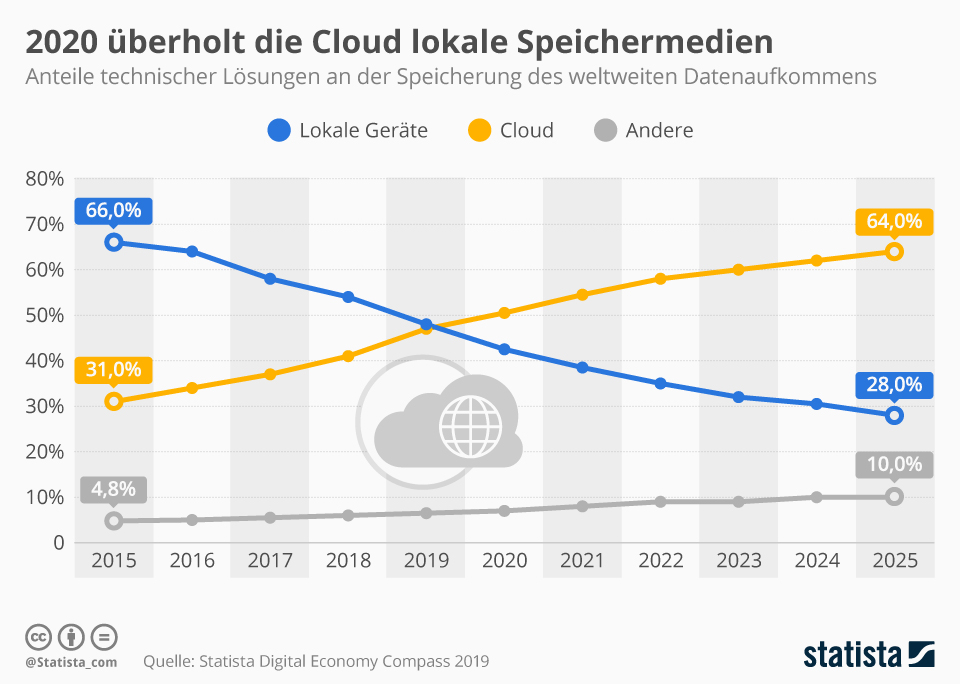
\includegraphics[scale=0.4]{sources/moreCloudStorageThanLocal}
      \caption[2020 überholt die Cloud lokale Speichermedien]{}\label{fig:moreCloudStorageThanLocal}
      2020 überholt die Cloud lokale Speichermedien, Statista, 2019 {\cite{STA1}}
\end{figure}
\\\\
\\\\
\\\\
Dieses grundlegende Kapitel hat einige potenzielle Vorteile der Nutzung von Cloud-Diensten für Unternehmen aufgezeigt. Darüber hinaus geht der Trend in den letzten Jahren zur Nutzung von Cloud-basierten Diensten. Das nächste Kapitel befasst sich mit den Zahlungsmodellen für EC2-Instanzen und den damit einhergehenden Abwägungen, die bei der Wahl dieser Modelle in verschiedenen Szenarien zu berücksichtigen sind.
\newpage

\begin{comment}
Advantages of Cloud Technology
As the technology has matured over the last decade, companies are moving to the
cloud to lower costs, reduce complexity, and increase flexibility. The cloud
provides scalable and powerful compute solutions, low-cost, reliable storage, and addition, cloud technologies can be used to deploy solutions quickly and cost effectively around the world and on any device.
When you decouple from the data center, you’ll be able to:
x Decrease your TCO: Eliminate many of the costs related to building and
maintaining a data center or colocation deployment. Pay for only the
resources you consume.

x Reduce complexity: Reduce the need to manage infrastructure,
investigate licensing issues, or divert resources.
x Adjust capacity on the fly: Add or reduce resources, depending on
seasonal business needs, using infrastructure that is secure, reliable, and
broadly accessible.
x Reduce time to market: Design and develop new IT projects faster.
x Deploy quickly, even worldwide: Deploy applications across multiple
geographic areas.
x Increase efficiencies: Use automation to reduce or eliminate IT
management activities that waste time and resources.
x Innovate more: Spin up a new server and try out an idea. Each project
moves through the funnel more quickly because the cloud makes it faster
(and cheaper) to deploy, test, and launch new products and services.
x Spend your resources strategically: Switch to a DevOps model to free
your IT staff from operations and maintenance that can be handled by the
cloud services provider.
x Enhance security: Spend less time conducting security reviews on
infrastructure. Mature cloud providers have teams of people who focus on
security, offering best practices to ensure you’re compliant, no matter what
your industry.
\end{comment}

%\subsection{Was ist EC2? To Review}\label{subsec_UabsGrund4}
%Man kann HW und SW auswählen


% Amazon video Cloud Eco.: https://www.youtube.com/watch?v=kUNBx1MTwxw
% short explaniation https://www.youtube.com/watch?v=RI9RTbXEjLc
%3- Hard and Soft Savings https://youtu.be/Q5wSvUVPyYY?t=316
% Suche ein Buch, mit info darüber!



\section{Zahlungsmodelle}\label{kap_zahlungsmodelle}
Die Nutzung von EC2-Instanzen ist mit einem Zahlungsmodell verbunden. Die Wahl des Zahlungsmodells ist von entscheidender Bedeutung, um den besten Preis für EC2-Instanzen zu erzielen.
%EC2 and RDS(DB) spend are often on of the main portions of your overall AWS Bill t.ly/Mqwn
Die von Amazon Web Services angebotenen Zahlungsmodelle werden im Folgenden dargestellt.
\\\\
Das \textit{On-Demand-Modell} beinhaltet keine langfristigen Verpflichtungen, es ist daher die teuerste Alternative, die auf Stundenbasis berechnet wird. Die Modelle \textit{Saving Plans} und \textit{reservierte Instanzen(Reserved Instances)}erfordern den Abschluss von Verträgen über ein oder drei Jahre, um günstige Preise zu erhalten. \textit{EC2-Spot-Instanzen} sind das kostengünstigste Modell, sie haben aber den Nachteil, dass ihre Verfügbarkeit nicht immer garantiert ist. Jedes Zahlungsmodell hat seine Vor- und Nachteile und eignet sich für unterschiedliche Anwendungsfälle. Gute Ergebnisse können auch durch die Kombination mehrerer Zahlungsmodelle erzielt werden. %SAG DER CLOUD-EXPERT/FIRMA
Dies wird in Unterkapitel \ref{sssec:AWS-EC2-Fleet} behandelt.
%[WIRD ES?]
\\\\
In dieser Arbeit wird nicht darauf eingegangen, wie die richtige Server-Instanz ausgewählt werden sollte, da die Auswahl von individuellen Anforderungen abhängt, die von Fall zu Fall unterschiedlich sind. Im Allgemeinen wird empfohlen, Instanzen so nahe wie möglich an den AWS-Diensten, mit denen sie kommunizieren werden, zu platzieren. %[IST DIESE ERKLÄRUNG NÖTIG?]
% Ressourcen vs Cloud-Dienste sollte gekläert werden
Die beste Leistung wird außerdem angestrebt, indem sich diese Instanzen in räumlicher Nähe zur Mehrzahl der Endnutzer, befinden. 
%Vor- und Nachteile noch tabellarisch aufzulisten??
%https://youtu.be/Q5wSvUVPyYY?t=678
%Excess capacity/Spot Instances
\subsection{On-Demand-Instanzen}
Bei diesem Zahlungsmodell besteht keine Notwendigkeit, ein festes Anfangsbudget festzulegen. Die Kosten richten sich nach dem Verbrauch auf der Grundlage der Nutzungsstunden. Dieses Modell eignet sich für Projekte, deren Entwicklung unvorhersehbar ist und die Möglichkeit besteht, dass das es in kurzer Zeit abgeschlossen sein wird, sodass es nicht Sinnvoll ist, eine langfristige Verpflichtung einzugehen.
\\\\
Die Preise beim dem On-Demand Zahlungsmodell variiert je nach Instanz Typ, Region und der übertragenen Datenmenge. Die aktuellen Preise für die verschiedenen Regionen sind auf der Amazon-Website in der Sektion EC2 - On-Demand-Preise\footnote{AWS On-Demand Instances Pricing.\cite{AMZ02}} zu finden. 
%Hierzu ein Beispiel für die Preise der EC2-Instanzen im On-Demand Zahlungsmodell.
\begin{figure}
    \centering
    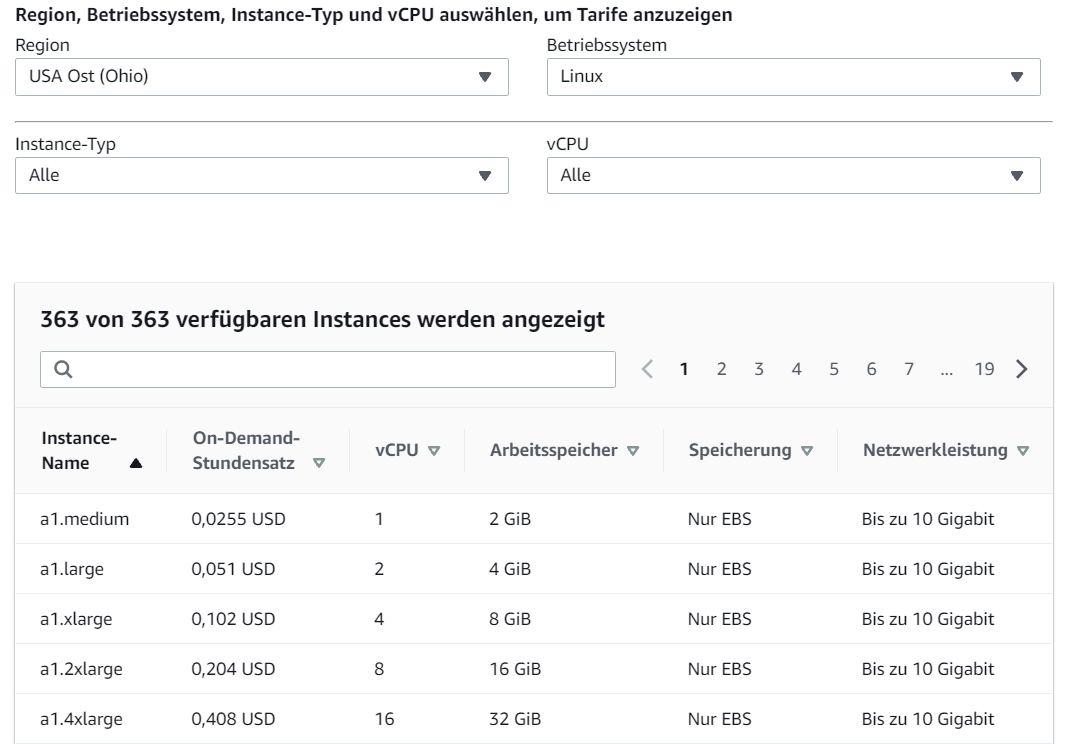
\includegraphics[scale=0.5]{sources/On-Demand-Pläne für Amazon EC2}\label{fig:OnDemand_Preise}\\
    \caption[On-Demand Preise für Amazon EC2]{}
    \label{fig:OnDemand_Preise}  On-Demand Preise für Amazon EC2 \footnote{\cite{AMZ02}}
  \end{figure}
In der \autoref{fig:OnDemand_Preise} werden die für die Region Ohio verfügbaren Linux-Instanzen gezeigt. Es ist zu beachten, dass Instanzen mit denselben Eigenschaften, aber in verschiedenen Regionen, unterschiedliche Preise haben können.
 %WARUM IST DIESE ABB.?
\subsection{Reservierte Instanzen und Saving Plans}
%t.ly/JUWq
%https://www.youtube.com/watch?v=c_zlPQimrvY
Die Zahlungsmodelle \textit{reservierte Instanzen} und \textit{Saving Plans} sind sich sehr ähnlich. Beide kommen mit einer gleichbleibenden  Nutzungsverpflichtung, die in €/Stunden gemessen wird. Um die reduzierten Preise  zu bekommen, müssen Verträge über ein oder drei Jahre abgeschlossen werden. 
\\\\
Die \autoref{fig:EinsparungenRISP} zeigt die möglichen Einsparungen je nach Zahlungsmodell. Die Einsparungen hängen mit der Flexibilität bei der Wahl der Instanzfamilie und der Verfügbarkeitszone zusammen, in die Instanzen übertragen werden können. Je geringer die Flexibilität, desto höher die Einsparungen.
\begin{figure}[h!]
  \centering
  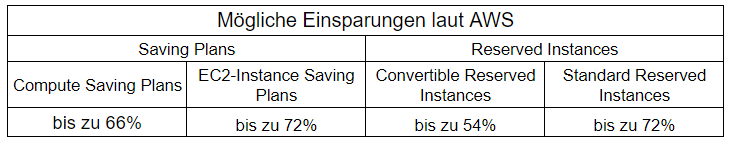
\includegraphics[scale=0.8]{sources/EinsparungenRISP}\label{fig:EinsparungenRISP}\\
  \caption[Mögliche Einsparungen bei reservierten Instanzen and Saving Plans laut AWS]{}
  \label{fig:EinsparungenRISP}
  Mögliche Einsparungen bei reservierten Instanzen and Saving Plans laut AWS
  \footnote{\cite{AMZ07,AMZ11}}
\end{figure}
\\
Compute Saving Plans\footnote{AWS Saving Plans Pricing\cite{AMZ11}.} bieten die Flexibilität EC2-Instanzen nach Familie\footnote{AWS Certified Solutions Architect - Associate (SAA-C02), S.95.\cite{AWS1}.}, Größe, Verfügbarkeitszone (AZ), Betriebssystem oder Mandant zu wechseln. Diese Option ist bei EC2-Instance Saving nicht möglich und daher bietet diese Alternative eine etwas höher Einsparung.
\begin{quote}
    „Bei Compute Saving Plans können Sie beispielsweise jederzeit von C4- auf M5-Instances wechseln, eine Workload von EU (Irland) nach EU (London) verlagern oder eine Workload von EC2 auf Fargate oder Lambda verschieben. Dabei zahlen Sie automatisch weiterhin den Saving Plans-Preis.”
    \footnote{AWS Saving Plans Pricing\cite{AMZ11}.}
\end{quote}
Bei den EC2-Instance Saving Plans hingegen muss eine Instance-Familie in einer bestimmten Region ausgewählt werden.  Dies reduziert automatisch die Kosten für die ausgewählte Instanz-Familie in der jeweiligen Region, unabhängig von Availability Zone, Größe, Betriebssystem oder Mandant.
%\\Die Festlegung eines festen Stundensatzes über einen langen Zeitraum bietet die Möglichkeit, künftige Kosten zu planen[ZITAT/WIE IM BWL ERKLÄRT]WIEDER EINBLENDEN; WENN ES SINNVOLL IST.
%-
%Folgenden Kriterien definieren den Preis von EC2-Instanzen bei SavingPlans:
%Vertraglaufzeit, Vorabzahlung, Betriebssystem,Region, Mandant
%AUCH FÜR RIs?
%3 Arten von S. Plans: Compute and EC2 Instance

%RI Configurations-Normalization https://medium.com/driven-by-code/how-truecar-saves-40-on-aws-with-ec2-reserved-instances-d0a6e0d9c08a
\subsubsection*{EC2 Reserved Instance Marketplace}\label{sssec:RI-Marketplace}
Sollte sich herausstellen, dass die Kapazität der reservierten Instanzen viel zu wenig oder gar nicht genutzt wird, kann diese Rechenkapazität auf dem \textit{RI Marketplace}(Marktplatz für den Kauf von reservierten Instanzen) zur Verfügung gestellt werden. Somit kann ein Teil der Investition zurückgeholt werden. Dies ist für Standard reservierten Instanzen möglich.
Diese Instanzen werden in Spot-Instanzen umgewandelt, damit andere Nutzer sie beantragen können. Dafür sollte eine Servicegebühr in Betracht gezogen werden. Stand November 2021 beträgt diese Gebühr 12\%\footnote{Amazon EC2 Reserved Instance Marketplace\cite{AMZ23}.}.

\subsubsection*{Möglichkeit der Vorauszahlung}\label{sssec:Vorauszahlung}
Zusätzlich gibt es bei Saving Plans und reservierten Instanzen die Option im Voraus zu zahlen. Im Gegenzug wird ein niedrigerer Preis angeboten. Amazon bietet drei verschiedene Optionen an. Diese sind eine teilweise, keine oder eine vollständige Vorauszahlung\footnote{ AWS Pricing Calculator\cite{AMZ17}.}. Bei teilweiser Vorauszahlung ist eine Anzahlung von etwa 50\% zu leisten.
\\\\
Die \autoref{fig:EinsparungenVorauszahlung} zeigt den Vergleich zwischen den drei Optionen für Vorauszahlungen. Hier wird deutlich, dass es kaum einen Unterschied zwischen eine teilweise Vorauszahlung und keine Vorauszahlung zu machen gibt. Eine erhebliche Einsparung ergibt sich, wenn man für den gesamten Zeitraum der gebuchten Instanzen im Voraus bezahlt.
\begin{figure}[h!]
    \centering
    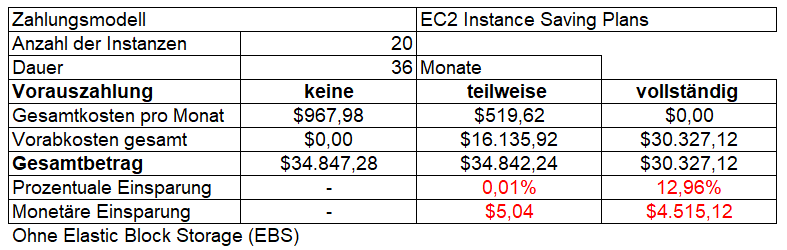
\includegraphics[scale=0.6]{sources/EinsparungenVorauszahlung}\label{fig:EinsparungenVorauszahlung}\\
    \caption[Mögliche Einsparungen durch Vorauszahlungen]{}
    \label{fig:EinsparungenVorauszahlung}Mögliche Einsparungen durch Vorauszahlungen für EC2 Instanzen in Saving Plans Zahlungsmodell\\
    Eigene Darstellung. Quelle: {AWS Pricing Calculator\cite{AMZ17}.}
  \end{figure}
  \\
Die Berechnungen wurden mit dem AWS Pricing Calculator {\cite{AMZ17}} für Instanzen der Familie t4g.xlarge, in der EU (Frankfurt) und für eine Laufzeit von 3 Jahren durchgeführt. 
\subsection{Spot Instanzen }\label{ssec:Spot-Instances}
Wie in Unterkapitel \ref{sssec:RI-Marketplace} genannt bieten EC2 Spot-Instanzen die Möglichkeit aus den ungenutzten EC2-Instanzen anderer Nutzer zu profitieren. 
Mit einem Preisvorteil von bis zu 90 \% gegenüber normalen On-Demand-Instanzen sind Spot-Instanzen ideal für fehlertolerante Anwendungen wie auf Containern ausgeführte Workloads, CI/CD, Bigdata-Anwendungen und ähnliches.

\subsubsection*{Unterbrechbarkeit}
Es ist zu beachten, dass Spot-Instanzen jederzeit unterbrochen werden können. Einer der Gründe ist die Preisüberschreitung der Instanz. Wenn Spot-Instanzen angefordert werden, wird einen Maximalpreis festgelegt. Ist der Preis der Spot-Instanz höher als der eingegebene Maximalpreis, ist die Spot-Instanz für die aktuelle Einstellung nicht mehr verfügbar. Ein anderes Szenario ist, wenn der Instanz Anbieter die Spot-Instanz erneut anfordert. Falls eine Spot-Instanz unterbrochen wird, benachrichtigt Amazon EC2 zwei Minuten im Voraus. Dieses Ereignis ist verfügbar auf CloudWatch, damit weitere Alarmen eingestellt werden. Diese und andere Funktionalitäten von CloudWatch werden in Kapitel \ref{kap_kostenüberwachung } näher erläutert.
\\
Da Spot-Instanzen anfällig für Unterbrechungen sind, ist es nicht empfehlenswert, für Produktionsumgebungen nur Spot-Instanzen zu verwenden.
%Um von der Preisvorteile der Spot-Instanzen zu profitieren und Ausfälle zu vermeiden, sollten in Kombination weitere Zahlungsmodelle verwenden werden.
%\\
%Zum Beispiel eine Kombination aus Spot-Instanzen für die erwarteten Last und On-Demand-Instanzen für die dynamischen Last.
%https://aws.amazon.com/de/ec2/spot/pricing/

%2 OPTIONEN: LOWEST PRICE OR DIVERSIFIED ACROSS n POOLS TO AVOID DOWNS https://www.linkedin.com/learning/aws-automation-and-optimization/request-spot-instances-part-2?autoAdvance=true&autoSkip=true&autoplay=true&resume=false&u=79182202

\subsection{Amazon EC2 Fleet[rev]} \label{sssec:AWS-EC2-Fleet}
\textit{Instanzen-Flotten} oder auf Englisch fleet of instances, bieten bei AWS die Möglichkeit mehrere Spot-Instanzen anzufordern, um einen bestimmten Bedarf an Rechenleistung zu decken\footnote{Amazon Elastic Compute Cloud - Benutzerhandbuch für Linux-Instances, S.708\cite{AMZ26}.}. Spot-Instanzen können auch für produktive Umgebungen verwendet werden\footnote{ Running Web Applications on Amazon EC2 Spot Instances\cite{AMZ24}.}. Darüber hinaus ist es empfehlenswert, Instanzen aus verschiedenen Zahlungsmodellen zu kombinieren, um von den Einsparungen von Spot-Instanzen, Saving Plans und reservierten Instanzen zu profitieren. Die Kombination von Instanzen aus verschiedenen Zahlungsmodellen beseitigt den Nachteil für Produktionsumgebungen, der mit Spot-Instanzen verbunden ist. Das heißt, das Risiko, dass Spot-Instanzen unterbrochen werden können.
\\\\
Folgende Punkte sind für die Nutzung von Spot Fleet Instanzen zu berücksichtigen:
\subsubsection*{Wahl der Spot-Instanzen[rev]}
Die Instanzen, die in der Auswahl für die Instanzen-Flotte berücksichtigt werden, müssen den Anforderungen der Applikation entsprechen. Um die Wahrscheinlichkeit zu erhöhen, dass mehr Spot-Instanzen gefunden werden, ist es empfehlenswert, die Kriterien der Suche zu erweitern. Dies kann erreicht werden, indem Instanzen ähnlicher Typen einbezogen werden. Die Berücksichtigung von Instanzen von Familien mit mehr Leistung als erforderlich, ist ebenfalls eine gute Option\cite{AMZ24}, da der Preis für Spot-Instanzen trotz höherer Leistung geringer sein wird als bei einem On-Demand Zahlungsmodell.
%Alte Version: . Denn, obwohl die Leistung die Anforderungen der Applikation überstiegen werden, wird es einen reduzierten Preis für die Spot-Instanzen bezahlt als bei On-Demand Zahlungsmodell.
\\\\
\subsubsection*{Maximaler Stundenpreis[rev]}
Wie im Unterkapitel \ref{ssec:Spot-Instances} erwähnt, muss für die Anforderung von Spot-Instanzen ein Maximalpreis festlegt werden. In diesem Fall ist die Festlegung dieses Maximalpreises auch für die gesamte Instanzen-Flotte eine Option. Es kann erwartet werden, dass die Spot-Preise im Laufe der Zeit stabil bleiben, da sie keinen starken Preisschwankungen unterliegen. Die aktuellen Preis und der Preisverlauf von Spot-Instanzen können in auf der AWS-Konsole\footnote{AWS EC2 Spot Instanzen-Anfragen und Preisverlauf\cite{AMZ25}.} abgefragt werden. Diese Informationen sind nur mit einem AWS-Konto zugänglich.
\\
\subsubsection*{Festlegung von On-Demand-Anteil[rev]}
Wenn alle oder eine große Anzahl von Spot-Instanzen nicht mehr verfügbar sind, muss die benötigte Rechenkapazität von Instanzen anderer Zahlungsmodellen wie On-Demand abgedeckt werden. Die Standardeinstellungen liegen bei 70\% On-Demand-Instanzen und 30\% Spot-Instanzen\cite{AMZ24}. Im Fall von vorhandenen reservierten Instanzen oder Instanzen von Saving Plans werden On-Demand-Instanzen zum entsprechend reduzierten Preis berechnet\footnote{Amazon Elastic Compute Cloud - Benutzerhandbuch für Linux-Instances, S.690\cite{AMZ26}.}.

\subsubsection*{Auto Scaling Groups}%Sarah 6.12
Auch als \textit{EC2-Auto-Scaling-Gruppe}(ASG) bezeichnet, ist diese für die Skalierung der zu startenden Instanzen verantwortlich. Dazu wird eine Startkonfiguration benötigt, welche definiert, unter welchen Bedingungen Instanzen gestartet oder beendet werden sollen[rev]. In der Startkonfiguration werden unter anderem der Instanztyp, Security-Groups, und Tags festgelegt. Mehr über Auto-Scaling und seine verschiedenen Konfigurationen in Kapitel~\ref{kap_Optimierung}.
\\\\
Für die Nutzung von EC2-Flotten und Auto Scaling-Gruppen fallen keine zusätzlichen Kosten an. Man muss nur für die durch die EC2-Instanzen verursachten Kosten bezahlen\footnote{Amazon Elastic Compute Cloud - Benutzerhandbuch für Linux-Instances, S.709\cite{AMZ26}. }. 
%\subsubsection*{Einschränkungen?[rev]}

\subsection{Anwendungsfall: TrueCar[rev]}\label{ssec:UseCaseTrueCar}
Instanzen in Zahlungsmodellen, die zu zeitlichen Verpflichtungen führen, bergen die Gefahr, dass die benötigte Rechenkapazität mittel- bis langfristig falsch eingeschätzt wird. Einerseits kann die reservierte Rechnerkapazität zu gering eingeschätzt werden. Als Konsequenz wird es großenteils der Rechnerkapazität mit On-Demand-Instanzen gedeckt, welche in dem Anteil der reservierten Instanzen berücksichtigt werden konnten und mit reduzierten Preisen berechnet. Andererseits, wenn zu viel Rechnerkapazität mit reservierten Instanzen reserviert und diese zu wenig gebraucht wird. Besteht die Möglichkeit, dass es die reine Nutzung von On-Demand-Instanzen eine kostengünstigere Option darstellt.
\\\\
Im Folgenden wird die Strategie beschrieben, dass\textit{TrueCar Inc}. verfolgt hat, um in keine der beiden oben genannten Situationen zu geraten. Dank ihrer Optimierungsstrategie konnten sie ihre AWS-Kosten durch die Nutzung reservierter Instanzen um etwa 40\% senken\footnote{How TrueCar Saves 40\% on AWS with EC2 Reserved Instances\cite{MED1}.}.
\\\\
Um Einsparungen von 40\% zu erreichen, musste das Team von TrueCar zuerst verstehen, wie AWS-Dienste wie reservierte Instanzen, Cost-Explorer, Auto-Scaling-Gruppen und Lambda Funktionen funktionieren. Damit haben sie eines der häufigsten Hindernisse überwunden, mit denen Unternehmen bei der Nutzung von Cloud-Diensten konfrontiert werden und zwar die Mangel an technisches Wissen in Bezug auf Cloud-Dienste\footnote{Accenture Dienstleistungen GmbH. Hohe Erwartungen an die Cloud: Hürden meistern, Mehrwert maximieren, S.11\cite{ACC1}.}. Nachdem das Team von TrueCar die notwendigen Informationen, insbesondere über die reservierten Instanzen, verstanden haben, haben sie die benötigte Rechenkapazität ermittelt. In dem Artikel wurde nicht erläutert, wie die von TrueCar benötigte Rechnerkapazität berechnet wurde. Diese Informationen werden jedoch von Cost-Explorer bereitgestellt. Cost-Explorer bietet die Möglichkeit, die Nutzung der AWS-Services für die letzten 12 Monate anzuzeigen. Cost-Explorer wird in Unterkapitel~\ref{ssec:Cost-Explorer} ausführlicher behandelt.
\\\\
Die Kosten der Instanzen in On-Demand wurden mit dem von reservierten Instanzen gegenübergestellt, um den Break-Even-Point dazwischen zu finden. Der Break-Even-Point bedeutet in diesem Fall, der Punkt, wo die Preise der reservierten Instanzen und die On-Demand Instanzen gleich sind. Nach diesem Punkt wird der monatliche Preis für die reservierten Instanzen sinken, bis die reservierte Kapazität verbraucht wird oder der Zeitraum für die reservierten Instanzen endet.
\\\\
Wie in der Grafik der \autoref{fig:Kosten_RIvsOn-Demand_pro_Monat_TrueCar} dargestellt wird liegt der Break-Even-Point zwischen dem Monat acht und neun. Im Fall, dass da Verbrauch der Instanzen vor dem Monat auch endet, würde, wäre es nicht empfehlenswert Instanzen zu reservieren, sondern mit On-Demand Instanzen zu arbeiten. Die Berechnung wurde gemacht für den Zeitraum von 1 Jahr durchgeführt. [RECHNEN UND ERKLÄREN?]. 
\begin{figure}[h!]
  \centering
  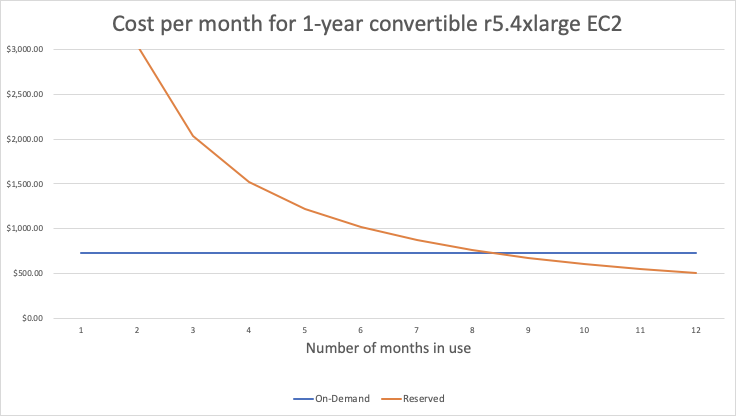
\includegraphics[scale=0.6]{sources/Kosten_RIvsOn-Demand_pro_Monat_TrueCar}\label{fig:Kosten_RIvsOn-Demand_pro_Monat_TrueCar}\\
  \caption[Monatliche Kosten für eine On-Demand-Instanz im Vergleich zu einer reservierten Instanz]{}
  \label{fig:Kosten_RIvsOn-Demand_pro_Monat_TrueCar}Monatliche Kosten für eine On-Demand-Instanz\\ im Vergleich zu einer reservierten Instanz.\\
  Quelle: Medium: How TrueCar Saves 40\% on AWS with EC2 Reserved Instances{\cite{MED1}}
\end{figure}
In dem Prozess wurden die Buchhaltungs- und Finanzabteilungen involviert[WICHTIG WEIL], um die Preisvorteile zu besprechen. Nach der Buchung der reservierten Instanzen wurde deren Nutzung mit Cost-Explorer überwacht. 
\\\\
Mit Cost-Explorer wurden die folgenden 2  Metriken überwacht: 
\\\\
\textbf{RI-Coverage}, die anzeigt, wie viel der On-Demand-Instanzen durch reservierten Instanzen abgedeckt wird. Ziel ist hierbei das RI-Coverage der reservierten Instanzen so nahe wie möglich an 100\% zu halten.
\\\\
\textbf{RI-Utilization}, welche zeigt, wie viel Prozent der reservierten Instanzen verbraucht wurden. Es wird versucht die RI-Utilization nicht zu niedrig zu halten.
\\\\
Um diese Metriken im Blick zu behalten und nicht jeden Tag den Cost-Explorer aufrufen zu müssen, wurde eine Benachrichtigung an Slack eingerichtet. Dies war über die Cost-Explorer API und eine Lambda-Funktion möglich.
\\\\
TrueCar, Inc. ist eine Preis- und Informations-Website für Neu- und Gebrauchtwagenkäufer mit Sitz in Santa Monica, Kalifornien\footnote{Die Quelle dieser Informationen ist ein Artikel, der auf https://www medium.com veröffentlicht wurde. Dass der Artikel von TrueCar stammt, wird durch die Tatsache bestätigt, dass deren Website https://www.truecar.com/who-we-are/ zu dem hier erwähnten Artikel führt.}.
%https://medium.com/driven-by-code/how-truecar-saves-40-on-aws-with-ec2-reserved-instances-d0a6e0d9c08a

\subsection*{Vergleich der Zahlungsmodelle[Rev]}
Die folgende Tabelle fasst die Eigenschaften der Zahlungsmodellen für On-Demand-, reservierte, von Saving Plans und Spot-Instanzen zusammen und listet typische Applikationen je nach Zahlungsmodell auf.
[Abb. VOLLSTÄNDIG?AKTUELL?]
\begin{figure}[h!]
    \centering
    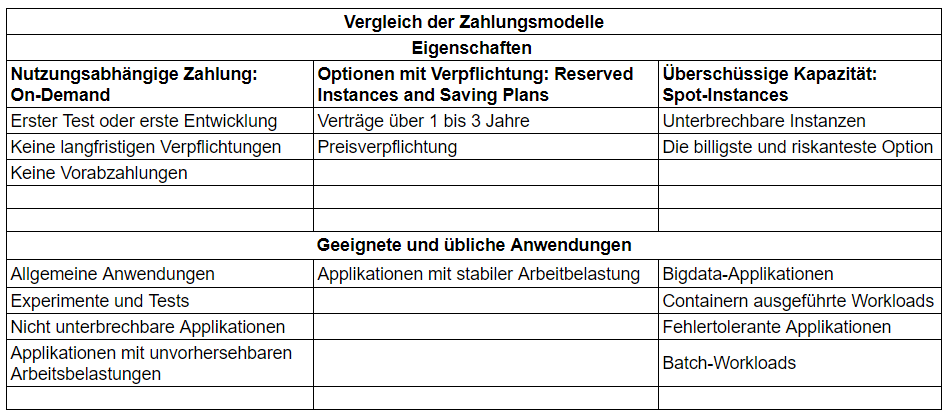
\includegraphics[scale=0.63]{sources/Vergleich_der_Zahlungsmodelle}\label{fig:Vergleich_der_Zahlungsmodelle}\\
    \caption[Vergleich der Zahlungsmodelle]{}
    \label{fig:Vergleich_der_Zahlungsmodelle}  Vergleich der Zahlungsmodelle nach Eingenschaft und Anwendungsfall\\
Eigene Darstellung. Quelle: {\cite{AMZ02, AMZ07, AMZ11, AMZ19,SPOT1}}\\
{Plusserver: Kostenoptimierung in AWS S.9.\cite{PS1}}
  \end{figure}
%
%To read planned at 21.11:
%https://www.pcapps.com/services/aws-reserved-vs-on-demand-instances/
%https://jaychapel.medium.com/aws-reserved-instances-versus-on-demand-which-is-better-e7f77f1f9582
%https://www.cloudhealthtech.com/blog/aws-reserved-instances-vs-on-demand#:~:text=In%20terms%20of%20compute%20options,of%20an%20On%20Demand%20instance.
%https://youtu.be/mKEdhmJ2udA?t=79
%Automate the selection to get the best price
%https://spot.io/aws-cost-optimization-calculator/

\newpage
\subsubsection*{Fazit[Rev]}
In diesem Kapitel wurden die verschiedenen Zahlungsmodelle für EC2-Instanzen untersucht. Es wurden Hinweise für die Auswahl des richtigen Zahlungsmodells in verschiedenen Szenarien gegeben. Dies wurde erklärt, um die Preisvorteile von den Zahlungsmodellen zu nutzen. Beginnend mit dem On-Demand-Zahlungsmodell, gefolgt von Reserved Instanzen und Saving Plans. In dieser Reihenfolge sinkt der Preis und mit ihm steigt die Verpflichtung, sich langfristig zu binden. Schließlich mit Spot-Instanzen, die die niedrigsten Preise bieten, aber keine volle Verfügbarkeit sicherstellen. %In Kapitel \ref{kap_Optimierung} wird weiter auf Optimierungsmaßnahmen für EC2-Instanzen durch den Einsatz von Auto Scaling Groups eingegangen.
\\\\
%[EC2-Fleet]
%En el capitulo monitoreo de costes  se mostrarán herramientas como X(CloudWatch) con las que podremos verificar si la desicion realizada fue la correcta. Para el modelo de pago On-Demand no hay ninguna redccion de los costos, pero existen medidas para aun asi reducir el uso de las instancias. Dichas medidas seran profundizadas en capitulo medidas de optimizacion
Im nächsten Kapitel wird CloudWatch[UND...] vorgestellt, mit dem überprüft werden kann, ob das ausgewählte Zahlungsmodell tatsächlich das Richtige für den betreffenden Anwendungsfall ist. [+Cost-Explorer+Trusted Advisor.] Für das On-Demand-Zahlungsmodell gibt es keine Kostenreduzierung, aber es gibt Maßnahmen, um die Nutzung von Instanzen zu reduzieren. Auf weitere Optimierungsmaßnahmen für EC2-Instanzen wird im Kapitel \ref{kap_Optimierung} näher eingegangen.
\newpage

\section{Kostenüberwachung}\label{kap_kostenueberwachung }
\input{chapters/Kostenüberwachung}
\newpage

\section{Optimierungsmaßnahmen}\label{kap_Optimierung}
%Cloud-Computing Basics a Non tech. intro.
%Seite 163
% Wie werden die Informationen die Benutzer gezeigt und wie können sie diese manipulieren
%[Rev]
Die mit den Überwachungswerkzeuge gesammelte Informationen, bilden die Grundlage für die Optimierungsmaßnahmen für EC2-Instanzen und Amazon S3.
%Wenn zum Beispiel festgestellt wird, dass Instanzen nicht ausreichend genutzt werden, können sie so konfiguriert werden, dass sie abgeschaltet werden.
%La mayoria de las medidas de opmimizacion se centran en las instancias EC2, pues como antes mencionado representan la gran mayoria de los servicios que comprenden los gastos en nuestras facturas.

\subsection{EC2 Auto Scaling}
%t.ly/CXs3 Linked In auf DE          %t.ly/1nka          %THIS!!! t.ly/vrCO
%https://youtu.be/qYHR_V1lvNU?t=900
Das \textit{Auto Scaling} oder die automatische Skalierung von Instanzen dient dazu die richtige Anzahl von EC2-Instanzen zur Verfügung zu haben, um die Anwendungslast dynamisch abzudecken.\footnote{Vgl. Was ist Amazon EC2 Auto Scaling? S.9\cite{AMZ31} } Diese Fähigkeit wird als \textit{horizontale Skalierung} bezeichnet.\footnote{Vgl. Die Grundbedeutung der horizontalen Skalierung ist, dass Systeme durch zusätzliche Komponenten erweitert werden. Im Gegensatz dazu bedeutet der Begriff "vertikale Skalierung", dass einer einzelnen Komponente zusätzliche Leistungsfähigkeiten und Ressourcen hinzugefügt werden. o.S.\cite{TECH1} }
\\\\
Die \autoref{fig:AutoSca_Unused_Capacity} zeigt das wechselnde Verhalten einer Beispielanwendung, die vor allem unter der Woche genutzt wird. Am Wochenende sinkt die Nachfrage nach Rechnerkapazität auf weniger als 25 \% und lässt den Rest der Kapazitäten ungenutzt. 
\begin{figure}[h]
    \centering
    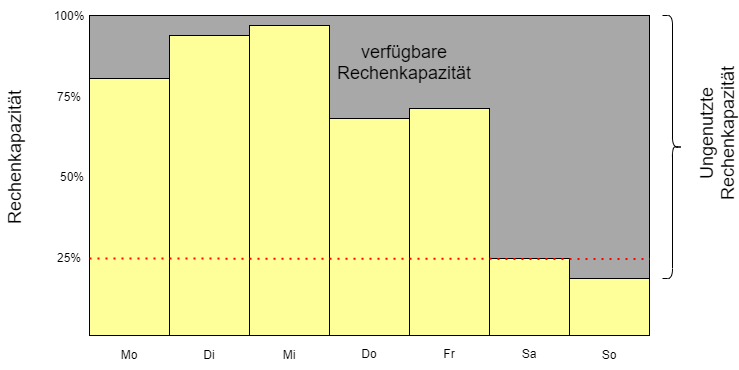
\includegraphics[scale=0.5]{sources/AutoCap Unused Capacity}
    \caption[Ungenutzte Rechenkapazität ohne automatische Skalierung]{}
    \label{fig:AutoSca_Unused_Capacity} Ungenutzte Rechenkapazität ohne automatische Skalierung. \\
    Quelle: Eigene Darstellung mit fiktiven Angaben. 
    %\footnote{\cite{AMZ01}}
  \end{figure}\\
Die gelben Säulen stellen die tägliche genutzte Rechenkapazität dar.
Die graue Zone entspricht ungenutzte Rechenkapazität und beträgt etwa ein Drittel der wöchentlichen Rechnerkapazität.
\subsubsection*{Auto Scaling Group}
Die Instanzen, die zur Deckung der erforderlichen Rechenkapazität zur Verfügung stehen, werden in einer \textit{Auto-Scaling-Gruppe(Auto Scaling Group)} zusammengefasst. Diese Gruppe von Instanzen wird in AWS als Auto-Scaling-Gruppe bezeichnet. Bei der Erstellung einer Auto-Scaling-Gruppe wird eine minimale, gewünschte und maximale Anzahl von Instanzen definiert. 
\\\\
Die \autoref{fig:BA Diagramme-AutoScaling and LoadBalancer.drawio} zeigt die gewünschte Instanzen einer Auto-Scaling-Gruppe, welche beim Start der Auto-Scaling-Gruppe gestartet werden. Die minimale und maximale Anzahl von Instanzen sind die Grenzwerte für die Auto-Scaling-Gruppe.  
\begin{figure}[h]
  \centering
  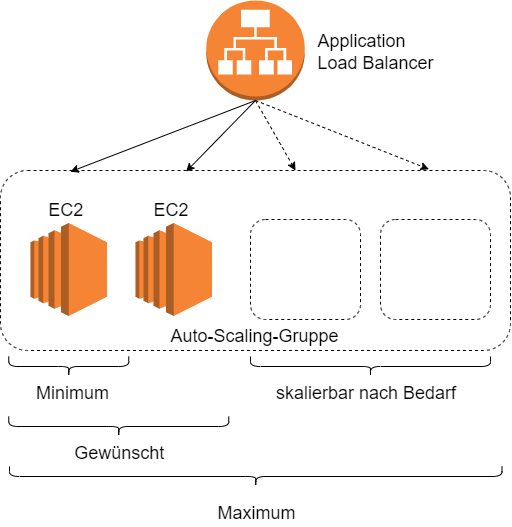
\includegraphics[scale=0.5]{sources/BA Diagramme-AutoScaling and LoadBalancer.drawio}
  \caption[Auto-Scaling-Gruppe nach den Anzahl der Instanzen und Umleitung der Datenverkehr durch dem Application Load Balancer]{}
  \label{fig:BA Diagramme-AutoScaling and LoadBalancer.drawio} 
  Auto-Scaling-Gruppe nach den Anzahl der Instanzen und\\ die Umleitung der Datenverkehr durch dem Application Load Balancer.\\
  Quelle: Eigene Darstellung %mit fiktiven Angaben. 
  basiert auf Amazon \\
  EC2 Auto Scaling - Benutzerhandbuch. S.9\cite{AMZ31}.
\end{figure}
%https://www.youtube.com/watch?v=yC5nRYS2IYI En Espaniol
%https://docs.aws.amazon.com/autoscaling/ec2/userguide/as-scaling-simple-step.html#policy-creating-asg-console
\\\\
%Zu erklären: cooldown period and scaling policy.
%Macht die Nutzung von Spor-Instanzen so einfach wie nie zuvor ?
\subsubsection*{Elastic Load Balancing}
%[Rev]
%https://docs.aws.amazon.com/autoscaling/ec2/userguide/autoscaling-load-balancer.html
%Durch einem \textit{Elastic Load Balancer} wird den eingehenden Anwendungsverkehr automatisch auf alle laufenden EC2-Instanzen verteilt. 
Ein \textit{Elastic Load Balancer} ist für die Verwaltung eingehender Anfragen zuständig, indem es den Datenverkehr auf alle laufenden EC2-Instanzen umleitet.\footnote{Vgl. In diesem Fall beschränkt auf den Application Load Balancer. Amazon Elastic Container Service Entwicklerhandbuch - Load Balancer-Typen - S.617\cite{AMZ39}} Dies sorgt dafür, Instanzen mit einem ausgeglichener CPU-Auslastung arbeiten. Die \autoref{fig:BA Diagramme-AutoScaling and LoadBalancer.drawio} zeigt einen Application-Load-Balancer, welcher den Datenverkehr auf die Instanzen einer Auto-Scaling-Gruppe verteilt.

\subsubsection{Zeitgesteuerte Skalierung}\label{ssec:ZeitgesteuerteScal}
%W-Ende für Dev und Beta
%\textbf{Nicht produktive Umgebungen}\\
%Auch möglich damit https://aws.amazon.com/de/solutions/implementations/instance-scheduler/
In einem On-Premise-System mache es, wenn überhaupt, einen kleinen Unterschied bei den Kosten, dass Instanzen die ganze Zeit aktiv bleiben.\footnote{Anders Lisdorf, 2021, S. 153\cite{CCB}} %\footnote{Vgl. ,Cloud Computing Basics: a Non.-Technical Introduction. Seite 153}. 
Im Gegensatz dazu ist es bei On-Demand-Zahlungsmodelle sinnvoll Zeiträume zu definieren, in denen Instanzen abgeschaltet werden können, um deren Nutzung zu reduzieren. Bei Systemen, die nur tagsüber und unter der Woche in Betrieb sein müssen, kann dies eine Einsparung von bis zu 67\% bedeuten. Wenn zum Beispiel Test- und Beta-Umgebungen von Montag bis Freitag von 7 bis 20 Uhr laufen würden. 
\\\\
Die \autoref{fig:Einsparung_Zeitgesteuerte_Skalierung} zeigt die Kostenberechnung einer nicht produktiven Umgebung (z.B. Test, Dev oder Beta) mit On-Demand-Instanzen. Diese Umgebung wird nur von Montag bis Freitag von 7:00 bis 20:00 Uhr genutzt. In der rechten Spalte werden die Kosten für Instanzen berechnet, wenn sie immer aktiv bleiben. In der linken Spalte wurde eine Berechnung durchgeführt, bei der die Instanzen nur dann eingeschaltet werden, wenn die Instanzen nach einem Zeitplan gesteuert würden.
\\\\
Die Abbildung zeigt am Ende den Prozentsatz und den Betrag(in Euros) der möglichen Einsparungen, wenn die Instanzen nach einer Zeitplan steuert werden würden.
\begin{figure}[h]
  \centering
  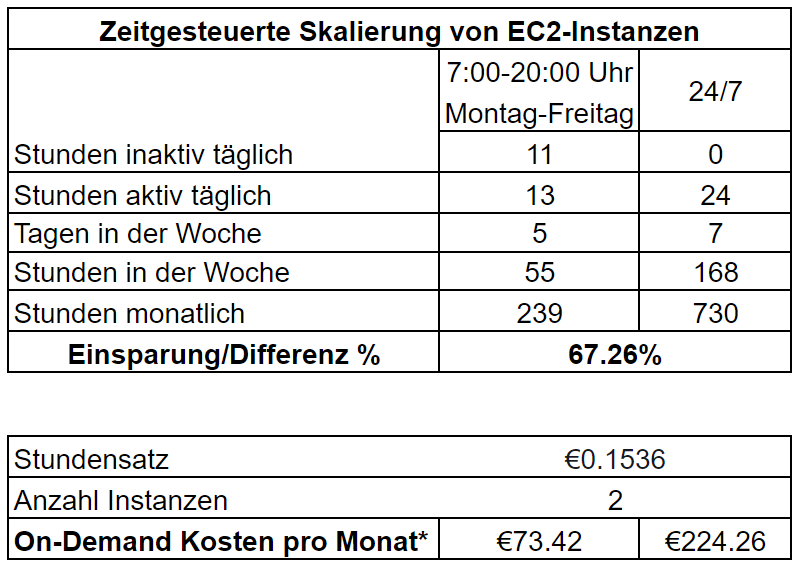
\includegraphics[scale=0.6]{sources/Einsparung_Zeitgesteuerte_Skalierung}
  \caption[Berechnung für ein nicht produktives Umgebung mit Zeitgesteuerte Skalierung]{}
  \label{fig:Einsparung_Zeitgesteuerte_Skalierung} 
  Berechnung für ein nicht-produktive Umgebung mit zeitgesteuerter Skalierung. \\
  Quelle: Eigene Darstellung.
\end{figure}
\\\\
\\\\
\\\\ 
Quelle des Stundensatzes: AWS Pricing Calculator.\footnote{Der Stundensatz wurde am 23.11.2021 mit dem AWS Pricing Calculator ermitellt für Linux Instanzen in Frankfurt mit 4vCPUs, 16 GB Arbeitsspeicher und Instanz-Familie t4g.xlarge in On-Demand-Zahlungsmodell\cite{AMZ17}.}
% Automatisiere das Hoch- und Herunterfahren von Instanzen
% https://www.linkedin.com/learning/monitoring-aws-with-cloudwatch/autoscaling-using-alarms?autoAdvance=true&autoSkip=true&autoplay=true&resume=false&u=79182202
% Grund: weil i.d.R., kein Entwickler 24/7 arbeitet.
% Wie?: mit Tagging, Lambda oder mit Auto Scaling Groups.
%Wann ist es sinnvoll Systeme runterzufahren 
%HIER LESEN {\cite{CCB}, Seite 153}
%Weihnachten und BackFriday
%\textbf{Produktive Umgebungen}\\
%Wenn der Zeitpunkt einer hohen Nachfrage bekannt ist, kann eine Erhöhung der Rechnerkapazität geplant werden, um Überlastungen zu vermeiden. Beispiele für solche Zeiträume sind Cyber-Monday und Black Friday\footnote{Vgl. Wie viel planen Sie am Black Friday / Cyber Monday auszugeben?\cite{STA5}}. 
%https://de.statista.com/statistik/daten/studie/1076963/umfrage/ausgaben-an-black-friday-und-cyber-monday-in-deutschland/]
\newpage
\subsubsection{Dynamisches Auto Scaling}
%[Rev]
%Intro mit Beispiel
Es kann jedoch zu schnelle und kontinuierliche Änderungen im Verhalten von Applikationen geben, häufig innerhalb von wenige Minuten. Bei solche Szenarien ist sinnvoller, Metriken zur automatischen Anpassung der Skalierung der Rechenkapazität festzulegen. Beispiele für eine veränderte Nutzung von Applikationen finden sich bei \textit{Tinder} und \textit{OkCupid}, zwei der größten Dating-Applikationen in den Vereinigten Staaten. 
\\\\
Die \autoref{fig:Use_by_hour_netflix_OkCupid_tinder} zeigt die Nutzungsspitzen bei den genannten Applikationen. Dieses wechselnde Verhalten wirkt sich unmittelbar auf die zu verschiedenen Tageszeiten benötigte Rechenkapazität aus und macht eine dynamische Skalierung der Rechenkapazität passend, wenn das Ziel darin besteht, ungenutzte Cloud-Dienste abzuschalten. Als Konsequenz der Abschaltung von ungenutzten Cloud-Diensten folgt die Reduzierung von Kosten.
\begin{figure}[h!]
  \centering
  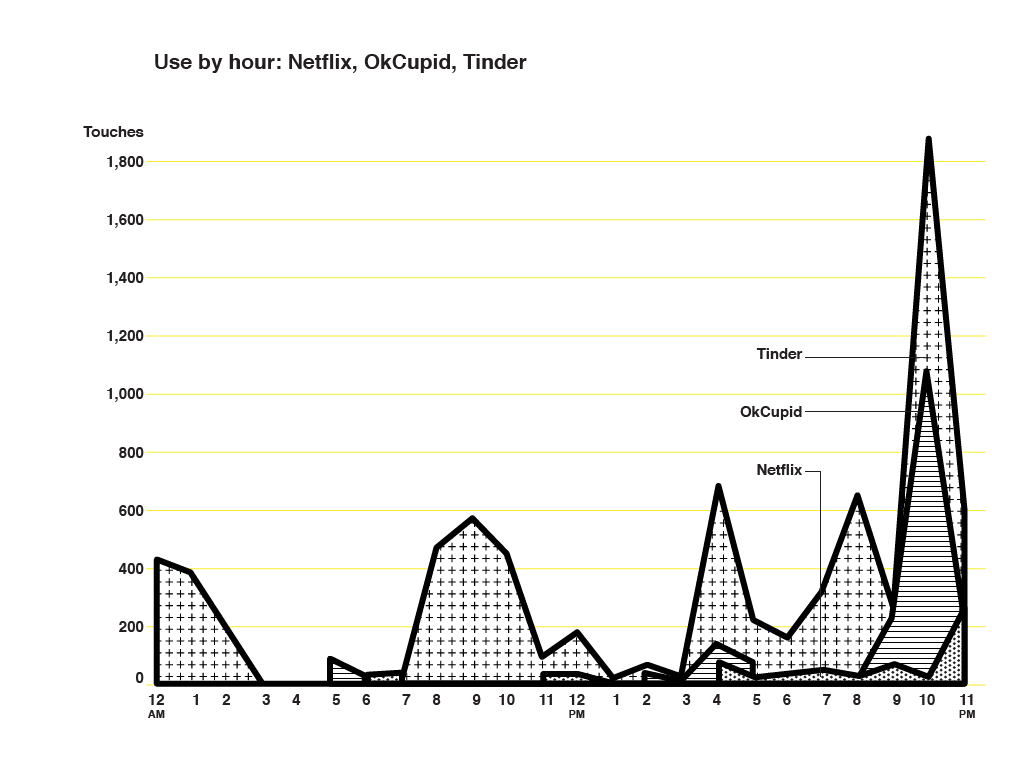
\includegraphics[scale=0.4]{sources/Use_by_hour_netflix_OkCupid_tinder}
  \caption[Nutzung von Tinder, OkCupid und Netflix pro Stunde]{}\label{fig:Use_by_hour_netflix_OkCupid_tinder} 
  DScout's Study: "Putting a Finger on Our Phone Obsession". \\
  Nutzung pro Stunde von Netflix, OkCupid und Tinder während des Tages\cite{SCOUT1}.
  %Quelle: Eigene Darstellung. 
  \\Mit Touches sind die Anzahl der Klicks, Swipes oder einfachen Interaktionen mit der Applikation gemeint.
\end{figure}
\\
Die für die automatische Skalierung erforderlichen Metriken wurden näher im Unterkapitel~\ref{ssec:CloudWatch} erwähnt. Eine der Metriken, die von AWS %[TELEFONAT mit Deepak von der Einheit CIS[Cloud Capgemini]]
benutzt wird, ist die gesamte CPU-Auslastung(CPU-Utilization). 
Um die CPU-Auslastung als Metrik zu verwenden, werden mindestens zwei Schwellenwerte definiert. Eine für die Erhöhung von Rechenkapazität, \textit{Scale-Out} genannt und eine für das Verringern von Rechenkapazität bezeichnet als \textit{Scale-In}.

\subsubsection{Manual Scaling}
%CHECK/23.11\\
Für die Konfiguration einer Auto-Scaling-Gruppe werden die minimale, maximale und gewünschte Anzahl von Instanzen definiert. Wenn aufgrund von Bedingungen, die in der Konfiguration einer Auto-Scaling-Gruppe nicht berücksichtigt wurden mehr oder weniger Rechenkapazität benötigt wird, ist es möglich, die Rechenkapazität manuell zu steuern. Dies geschieht, ohne dass die aktiven Instanzen unterbrochen werden.

\subsubsection{Predective Scaling}%Voraussagende Skalierung / 
Voraussagende Skalierung oder Predictive Scaling auf Englisch, nutzt maschinelles Lernen, um den Kapazitätsbedarf auf der Grundlage historischer Daten von CloudWatch vorherzusagen. Mit Hilfe der Predictive Scaling kann es die Kapazität vor der erwarteten Auslastung bereitstellen, im Gegensatz zur dynamischen Skalierung, die reaktiv ist. 
Für Instanzen, die viel Zeit für die Initialisierung benötigen, kann die Zeit zwischen dem Beginn des Nachfrageanstiegs und der Initialisierung der Instanz vermieden oder verkürzt werden.
%[(EIGENES) DIAGRAMM?]
Anders als Zeitgesteuerte Skalierung ist es nicht notwendig, die Verhaltensmuster der Anwendungen zu analysieren.
%[SOLLTE DAS ZITIERT WERDEN?]
%https://docs.aws.amazon.com/autoscaling/ec2/userguide/as-dg.pdf#ec2-auto-scaling-predictive-scaling

\subsection{S3 Optimierung}
In diesem Unterkapitel werden Maßnahmen zur Speicheroptimierung für Amazon S3 beschrieben. Jedem Objekt in Amazon S3 ist eine Speicherklasse zugewiesen. Die Speicherklassen werden nach der Zugriffshäufigkeit auf die Objekte unterschieden und sind für verschiedene Szenarien konzipiert. Es gibt Speicherklassen für den häufigen und den seltenen Zugriff.\footnote{Vgl. AWS: Amazon Simple Storage Service - User Guide. S.709.\cite{AMZ18}} Der Preis bei Amazon S3 wird pro GB berechnet und ist umso niedriger, je geringer der Zugriff auf die Objekte ist.\footnote{Vgl. AWS S3 Pricing \cite{AMZ09}} Um die Speicherkosten zu optimieren, ist es daher notwendig, die richtige Speicherklassen für die jeweilige Applikation zu wählen, weil die Speicherkosten durch ihre Klasse berechnet werden.

\subsubsection{Die richtige Speicherklassen wählen}%[Rev]
Um die richtige Wahl zu treffen, müssen die Anforderungen der Applikation verstanden werden. Ärztliche Patientenakten und \textit{Instagram-Stories} sind zwei Beispiele für Daten, die nach deren Erstellung für einen Mindestzeitraum oder auf unbestimmte Zeit aufbewahrt %und nicht gelöscht 
werden.\footnote{Vgl. Bei Instagram Stories handelt es sich um kurzen visuellen Content in der Regel Bilder oder kurze Videos, die nach 24 Stunden automatisch aus der Applikation Instagram verschwinden(Stand November 2021).\cite{IG2}} In Deutschland müssen ärztliche Patientenakten mindesten zehn Jahre aufbewahrt werden.\footnote{Vgl. Nach dem Bürgerlichen Gesetzbuch (BGB) § 630f müssen Patientenakten zehn Jahren nach Abschluss der Behandlung aufbewahrt werden, soweit nicht nach anderen Vorschriften andere Aufbewahrungsfristen bestehen. \cite{BGB}} \textit{Instagram} verwendet die von seinen Nutzern bereitgestellten Informationen, einschließlich der Metadaten von Bildern, um andere Instagram- und \textit{Facebook}-Produkte zu empfehlen.\footnote{Vgl. Instagram macht keine genauen Angaben darüber, wie lange die Nutzerdaten aufbewahrt werden, sondern gibt nur an, dass sie so lange wie nötig aufbewahrt werden. Hilfebereich Instagram: VII. Datenspeicherung, Deaktivierung und Löschung von Konten\cite{IG3}.}
%[nicht gelöscht, sondern archiviert]Im Gegensatz dazu wird eine Instagram-Story innerhalb von 24 Stunden von der Applikation verschwinden und archiviert\footnote{Vgl. Instagram: Wann verschwindet meine Instagram Story?\cite{IG1}}.
Die Zugriffshäufigkeit und die Aufbewahrungszeit sind die zwei Hauptkriterien für die Verschiebung von Daten zwischen Speicherklassen.\footnote{Vgl. AWS: Amazon Simple Storage Service - User Guide. S.711.\cite{AMZ18}}
\\\\
%AWS bietet verschiedene Speicherklassen an, die sich im Preis und in der Häufigkeit des Zugriffs auf die Objekte unterscheiden. 
%([Rev] UMFORMULIEREN :)
Objekte werden in Behältern gespeichert, die Buckets genannt werden. Daten werden über einen längeren Zeitraum gespeichert aufgrund der vorgeschriebenen Anforderungen oder weil per Gesetz auf die Informationen in der Zukunft zugegriffen werden muss.
%\\
Zusätzlich, wenn auf die Daten nicht häufig zugegriffen wird, sind Glacier und Glacier Deep Archive passende Speicherklassen. Die Entscheidung für eine bestimmte Speicherklasse ist jedoch nicht immer so leicht zu treffen. % jedoch die Umstände können sich schnell ändern. 
Hinzu kommt, dass nicht alle Daten in einer Applikation immer die gleichen Zugriffsmuster haben. Für solche Fälle ist es möglich, Regeln zu definieren, die Dateien zwischen verschiedenen Speicherklassen abhängig von ihrem Alter verschieben.
\newpage
\subsubsection{Lebenszyklus-Konfiguration}\label{ssec:Lebenszyklus-Konfiguration}
Die \textit{Lebenszyklus-Konfiguration} oder \textit{lifecycle policy} ist eine Maßnahme zur Optimierung für Amazon S3-Speichereinheiten. Eine S3-Lebenszykluskonfiguration beschreibt in einer XML-Datei Regeln und Aktionen für die Verschiebung in unterschiedlichen Speicherklassen von Objekten. Die Verschiebung von Objekten verursachen Kosten. Ein Beispiel von diesen Kosten und mögliche Einsparungen werden in \autoref{fig:Kostenvergleich_Nutzung_unt_Speicherklassen} vorgestellt.
\\\\
%Beim Verschieben nach S3 Intelligent-Tiering, S3 Standard – Infrequent Access und S3 One Zone – Infrequent Access: %\$0.01\\
%S3 Glacier: \$0.036\\
%S3 Glacier Deep Archiv: \$0.06\\
%Datenabfrage am 24.11.2
%{\cite{AMZ09}}
%\\
Um konkretere Regeln zu zu definieren, ist es möglich Tags zu verwenden und somit eine Unterscheidung zwischen Objekten mit verschiedenen Tags zu treffen. Es ist wie in dem folgenden Beispiel möglich, alle Objekte mit dem Tag-Wert: \textit{Dev} nach 45 Tagen nach Standard Infrequent Access und nach 120 Tagen nach S3 Glacier zu verschieben.
\begin{lstlisting}
  <LifecycleConfiguration>
  <Rule>
    <ID>example-id</ID>
 <Filter>
      <Tag>
         <Key>key</Key>
         <Value>Dev</Value>
      </Tag>
</Filter>
    <Status>Enabled</Status>
    <Transition>
      <Days>45</Days>
      <StorageClass>STANDARD_IA</StorageClass>
    </Transition>
    <Transition>
      <Days>120</Days>
      <StorageClass>GLACIER</StorageClass>
    </Transition>
    <Expiration>
      <Days>365</Days>
    </Expiration>
  </Rule>
</LifecycleConfiguration>

Angepasster Code auf Basis der Beispiele auf Seite 701 in 
Amazon Simple Storage Service - User Guide. 
\end{lstlisting}
\footnote{Vgl. AWS: Amazon Simple Storage Service - User Guide. S.701.\cite{AMZ18}}\\

\subsubsection{Anwendungsbeispiel für eine Lebenszyklus-Konfiguration}\label{Anwendungsbeispiel-Leben-Konfig}
Zur Veranschaulichung der Verschiebung von Objekten zwischen Speicherklassen wird der folgende Anwendungsfall vorgestellt. In diesem Fall wird der Punkt als Dezimaltrennzeichen und das Komma als Tausendertrennzeichen verwendet. 
\\\\
Ein Sicherheitsunternehmen muss Sicherheitsvideos speichern, die aktuell im Summe 120 TB groß sind. Viele von ihnen werden mindestens 5 Jahre lang aufbewahrt, falls sie vor Gericht als Beweismittel dienen sollten. Ungefähr 50\% der Videos werden mindestens einmal im Monat überprüft und müssen laut Gesetz sofort zugänglich sein. Die Software des Unternehmens speichert die Videos in S3-Buckets. Jedes Video hat eine durchschnittliche Größe von 3.4 GB.
\\\\
Im Folgenden werden die Speicherkosten für ein Szenario berechnet, bei dem nur \textit{S3 Standard} verwendet wird. Als nächstes wird die Kombination von \textit{S3 Standard Infrequent Access, S3 Glacier} und \textit{S3 Standard} für ein zweites Szenario betrachtet, in dem die Videos je nach Alter verschoben werden. Im zweiten Szenario müssen die Kosten für die Verschiebung zwischen Speicherklassen berücksichtigt werden. Die Verschiebung erfolgt durch eine Lebenszyklus-Konfiguration wie in der Unterkapitel \ref{ssec:Lebenszyklus-Konfiguration} beschrieben. Zum besseren Verständnis wird angenommen, dass 20\% der Dateien in S3 Standard Infrequent Access und 30\% in S3 Glacier gespeichert werden.
\newpage
\begin{figure}[h!]
  \centering
  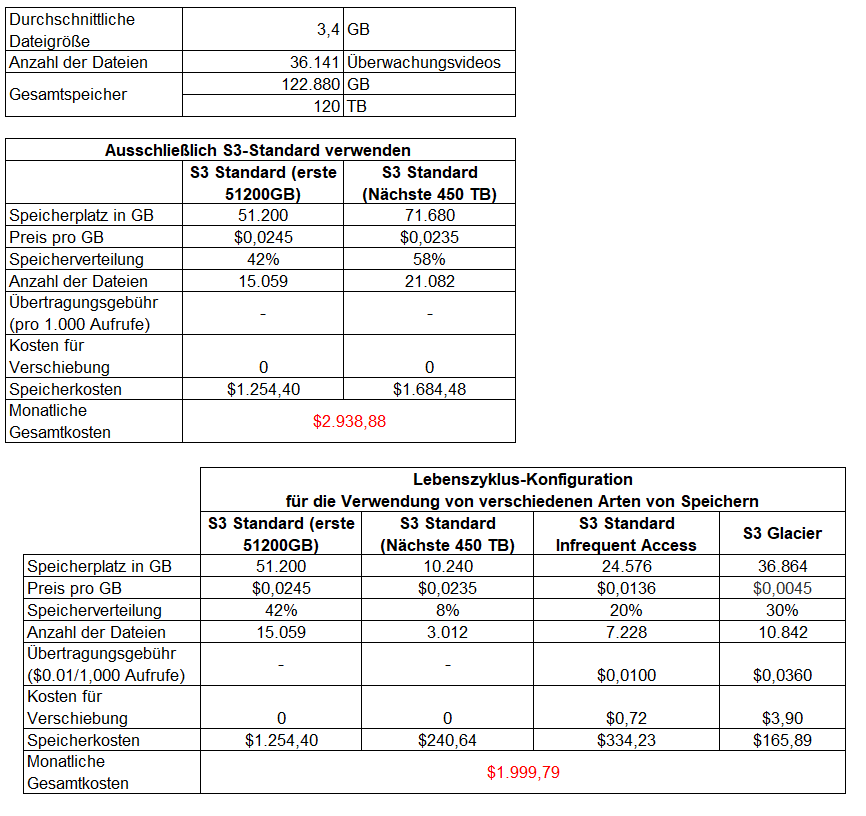
\includegraphics[scale=0.75]{sources/Kostenvergleich_Nutzung_unt_Speicherklassen}
  \caption[Kostenvergleich durch Nutzung von unterschiedlichen Speicherklassen]{}\label{fig:Kostenvergleich_Nutzung_unt_Speicherklassen} 
  Kostenvergleich durch Nutzung von unterschiedlichen Speicherklassen.  
\end{figure}
%\\
Quelle: Eigene Darstellung mit Stundensätze der S3-Preise.\footnote{Vgl. AWS S3 Pricing\cite{AMZ09}}
\\\\
Bei der Berechnung wurden die Kosten für das Verschieben von Videos zwischen Speicherklassen berücksichtigt. Anhand der Berechnungen in der \autoref{fig:Kostenvergleich_Nutzung_unt_Speicherklassen} lässt sich erkennen, dass ein Einsparungspotenzial von rund 1,000(Eintausend) USD pro Monat besteht, indem die notwendigen Regeln aufgestellt werden, um einen Teil der Videos in anderen Speicherklassen zu verschieben, welche niedrigere Preise bieten.
%WICHTIG IST DIE GRÖSSE MEINE DATEIEN UND DIE ANZAHL.
%weil SO WERDEN DIE PREISE FÜR VERSCHIEBUNG BERECHNET.
%(Object size distribution )
\newpage
\subsubsection{Intelligent-Tiering}
\textit{Intelligent-Tiering} verschiebt Objekte auf der Grundlage von Zugriffsmustern. Diese Speicherklasse ist ideal für Objekte mit wechselnden oder unbekannten Zugriffsmustern. Wie die Senior Product Managerin für S3 Ruhi Dang erklärt, haben einige Unternehmen weder die Zeit noch das Geld, um eine Person einzustellen, die ihre Daten sortiert und in die richtige Speicherklasse einordnet. Intelligent Auto Tiering ist eine attraktive Lösung für Unternehmen, die jährlich weniger als 100,000 USD für Speicher ausgeben. \footnote{Vgl. Ruhi Dang, 2019, AWS re:Invent 2019: Guidelines and design patterns for optimizing cost in Amazon S3. Minute: 21:12 \cite{AMZ16}}
%Ach von Jessie Felix gesagt https://www.youtube.com/watch?v=IOT41L_adSw
%\\\\
Die \autoref{fig:S3_IntLifeCycle} zeigt, wie Objekte in Abhängigkeit davon, ob auf sie zugegriffen wurde oder nicht, verschieben werden. 
\begin{figure}[h!]
  \centering
  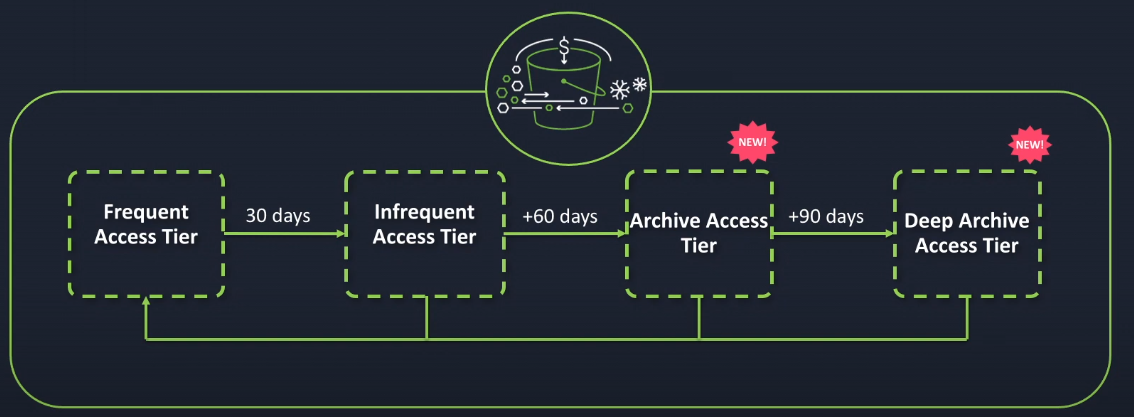
\includegraphics[scale=0.7]{sources/S3_IntLifeCycle}
  \caption[Funktionsweise von Intelligent-Tiering]{}\label{fig:S3_IntLifeCycle} Funktionsweise von Intelligent-Tiering
  %{\cite{SCOUT1}}
\end{figure}\\
Quelle: Eigene Darstellung auf der Grundlage von \\
der Funktionsweise von Intelligent-Tiering.\footnote{Vgl. Amazon Simple Storage Service - User Guide. S.715\cite{AMZ18}}
\\\\
Wird ein Objekt zu einem späteren Zeitpunkt aus der Ebene der seltenen Zugriffe aufgerufen, wird dieses automatisch in eine Speicherklasse der häufigen Zugriffe zurückversetzt.
%TALVEZ PARA RELLENAR UN POCO HACER UN CALCULO DE CUANTO SALDRIA SI SE USA Intelligent-Tiering para el caso de los videos
%En comparación con Lebenszyklus-Konfiguration Intelligent-Tiering objetos son regresados al ser llamados/usados.
%Ademas los tiempos de desplazamientos ya están definidos en Intelligent-Tiering.
\\\\
%Anwenfungsbeispiel?
Das in Unterkapitel \ref{Anwendungsbeispiel-Leben-Konfig} dargestellte Szenario wurde mit dem AWS Pricing-Calculator für S3 unter Verwendung der Speicherklasse S3 Intelligent-Tiering berechnet.\footnote{Vgl.  AWS Pricing Calculator S3\cite{AMZ17-S3}.}%Intelligent-Tiering bietet die Möglichkeit, Objekte in fünf verschiedenen Ebenen zu verschieben. 
Da bei der Berechnung des Unterkapitels \ref{Anwendungsbeispiel-Leben-Konfig} eine Speicherklasse für häufigen Zugriff, eine für seltenen Zugriff und eine für Archivierung verwendet wurde, wurden für die Berechnung mit Intelligent-Tiering vergleichbare Speicherebenen ausgewählt. In diesem Fall wurden ausschließlich die Ebenen \textit{Frequent-Access, Infrequent-Access} und \textit{Instant-Archive-Access} ausgewählt. %Die Ebenen \textit{Archive-Access} und \textit{Deep-Archive-Access} wurden vernachlässigt. %nicht berücksichtigt
\\\\
Die Speicherzuweisung für die 120 TB in den Speicherebenen war wie folgt:\\
Frequent-Access-Tier: 50\% \\
Infrequent-Access-Tier: 20\%\\
Instant-Archive-Access: 30\%
\\
\begin{figure}[h!]
  \centering
  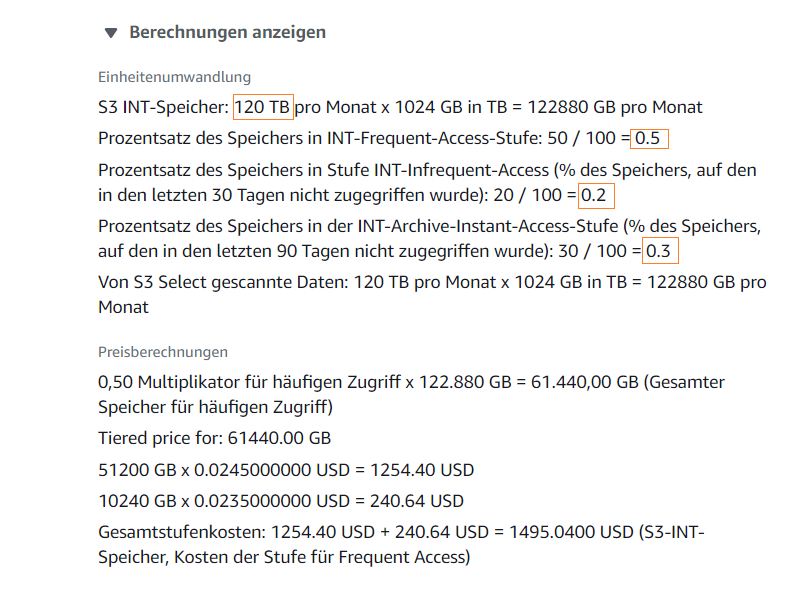
\includegraphics[scale=0.6]{sources/S3_INT_1}
  \caption[Berechnung für die Verwaltung von 120 TB mit AWS Pricing-Calculator für S3 Intelligent-Tiering(1)]{}
  \label{fig:INT_S3_1} Berechnung für die Verwaltung von 120 TB mit AWS Pricing-Calculator für S3 Intelligent-Tiering(1).\\
  Quelle: eigene Darstellung von AWS Pricing-Calculator \cite{AMZ17-S3}.
  %{\cite{SCOUT1}}
\end{figure}
\newpage
In der \autoref{fig:INT_S3_2} werden die Kosten gezeigt, die durch jede Speicherebene anfallen (mit orange markiert). 
\\
Darüber hinaus werden die folgenden Kosten berechnet (mit blau markiert): \\
- Überwachung und Automatisierung von 36.141 Objekten.\\
- Leseanfragen (GET-Anfragen) von 18.070 Objekten, welche 50\% der Gesamtzahl der Videos entsprechen, wie in den Anforderungen im Unterkapitel \ref{Anwendungsbeispiel-Leben-Konfig} definiert. \\
- Scannen von Objekten, die allen Videos und 120 TB entsprechen.
\\
\begin{figure}[h!]
  \centering
  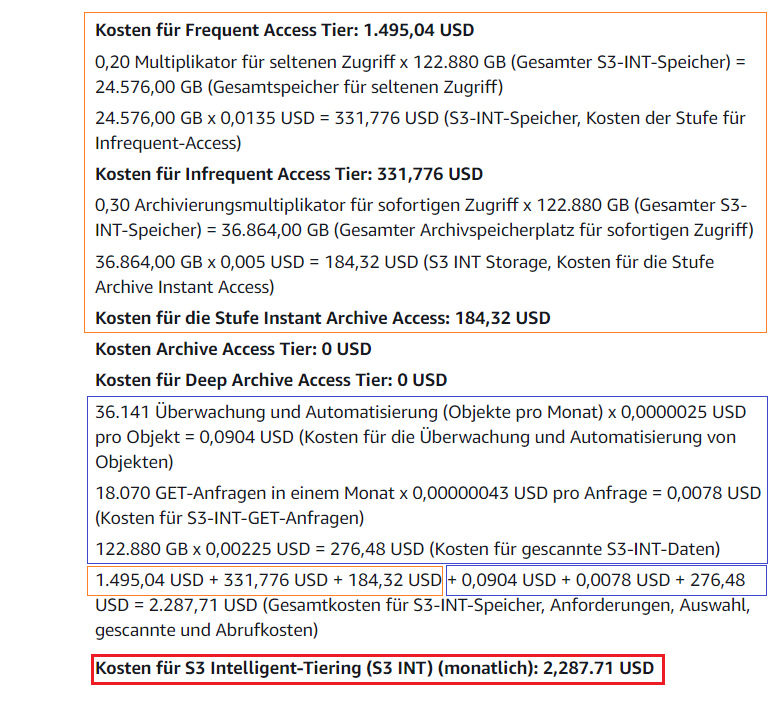
\includegraphics[scale=0.6]{sources/S3_INT_2}
  \caption[Berechnung für die Verwaltung von 120 TB mit AWS Pricing-Calculator für S3 Intelligent-Tiering(2)]{}
  \label{fig:INT_S3_2} Berechnung für die Verwaltung von 120 TB mit\\ AWS Pricing-Calculator für S3 Intelligent-Tiering(2).\\
  Quelle: eigene Darstellung mit AWS Pricing-Calculator \cite{AMZ17-S3}.
\end{figure}
\\\\
\subsubsection*{Unterscheidung zwischen Intelligent-Tiering und Lebenszyklus-Konfiguration}%[Rev]
Ein Unterschied zwischen der Verwendung von Intelligent-Tiering und einer Lebenszyklus-Konfiguration besteht darin, dass bei Intelligent-Tiering die Objekte in Ebenen von seltenen Zugriff automatisch auf eine Ebene für häufigen Zugriff zurückgegeben werden. Siehe \autoref{fig:S3_IntLifeCycle}.
\\\\
Ein weiterer Unterschied ist, dass bei einer Lebenszyklus-Konfiguration die Tage der Verschiebung zwischen den Speicherklassen und die Speicherklassen leicht verändert werden können. Dies ist standardmäßig bei Intelligent-Tiering bereits festgelegt. %Die Möglichkeit die Zeitabstand für die Verschiebung zwischen Ebenen bei Intelligent-Tiering wurde in der AWS-Dokumentation nicht gefunden. 
\\
Es gibt jedoch die Möglichkeit, Objekte aus Intelligent-Tiering in andere Speicherklassen zu verschieben (mit Einschränkungen), indem man eine Lebenszyklus-Konfiguration verwendet.\footnote{Vgl. AWS: Amazon Simple Storage Service - User Guide. S.724.\cite{AMZ18}} %t.ly/1CgV
Dies gäbe die Möglichkeit, Objekte für einen längeren Zeitraum in einer bestimmten Speicherklasse aufzubewahren und Richlinien von Intelligent-Tiering zu überspringen.
%COMMENTS
\begin{comment}
\subsubsection{Automatisierung mit Lambda Funktionen}
Grund: einmal programmiert, funktioniert es für immer.
\\(To-Do:) Möglichkeiten untersuchen, bewerten und die passende Auswählen.

%Limitierung 
%Quotas setzen? erweitern oder reduzieren / benachrichtigen aber auch eine Aktion durchführen 

%Lambda

AWS Lambda is a compute service. You can use it to run code without provisioning or managing servers. Lambda runs your code on a high-availability compute infrastructure. It operates and maintains all of the compute resources, including server and operating system maintenance, capacity provisioning and automatic scaling, code monitoring, and logging. With Lambda, you can run code for almost any type of application or backend service. 

Some benefits of using Lambda include the following:

You can run code without provisioning or maintaining servers.
It initiates functions for you in response to events.
It scales automatically.
It provides built-in code monitoring and logging via Amazon CloudWatch.
\end{comment}

%Data Pipeline

%Economic Performance?
%QUEUES

%NEVER forget your availability requirements, trying to optimize, first availability THEN cost...
%Do not use your DB for saving BLOB

%\subsection{VERKAUFE DEINE Ungenutzte Kapazität in RI Marketplace}

%Kombination
%https://spot.io/blog/effective-utilization-of-aws-savings-plans-and-ec2-spot-instances/#a1
%https://www.youtube.com/watch?v=X_7pnzPlESs

 
\newpage

\section*{Zusammenfassung}\label{kap_zusammfAusbl}
\addcontentsline{toc}{section}{Zusammenfassung} % Manuellen Eintrag im Inhaltsverzeichnis erzeugen
(To-Do:)
\\Kapitelweise Kurzdarstellung der Inhalte (inklusive Referenzierung auf die \\Kapitelnummerierung) => Nach dem Motto: \textit{Was wurde wo beschrieben?}
\\Kurzdarstellung \textit{Problem – Lösungsweg – Ergebnisse}
\\Rückkopplung auf die Einleitung: Wurde die Zielstellung der Arbeit und die \\Fragestellung zufriedenstellend beantwortet?
\\Kritische Bewertung (sofern nicht bereits im Hauptteil geschehen)
\\Offene Probleme
\\Richtung der zukünftigen/möglichen Arbeiten
\\Erläuterung, warum welche Aspekte in der Arbeit nicht erläutert 

\subsection{Umweltbezogene Aspekte}
Esta tesis habla sobre monitoreo y optimizacion de recursos de manera financiera. Pero esas dos areas enfocadas a la economia, tiene impacto en el medio ambiente por las emisiones generadas por las granjas de servidores. 
Estadisticas dicen que en Europa/Alemania se generan x toneladas de CO2 provenientes de centros de computo. Por tanto al monitoreat y reducir cosotos, se estan evitando despilfarros y al final tambien emisiones de CO2. 
\\
\subsection{Test von den Werkzeugen und Maßnahmen}
Da es in dieser Arbeit zeitlich nicht gelungen ist, die Überwachungswerkzeuge und Optimierungsmaßnahmen umzusetzen, bleibt es noch sie in einer echten Umgebung zu testen. Es wäre möglich zu verifizieren, ob die hier genannten Maßnahmen zur vergleichbaren Einsparungen führen, wie die vom Cloud-Anbieter Amazon genannten.

Amazon bietet ein kostenloses Kontingent an, die jedoch für diese Tests nicht genug war. 
\\
\subsection{Bewusstsein in der gesamten Organisation}
Zusätzlich zu den bisher genannten Maßnahmen ist es wichtig, dass Verbraucher von Cloud-Diensten Bewusstsein für die Entstehung von Kosten entwikclen.[ODER sensibilisier werden?] Von dem Entwickler bis zum der IT-Manager, jeder sollte wissen, dass es so einfach ist, Cloud-Dienste mit ein paar Klicks zu beauftragen. Diese können in kurzer Zeit ungewünschte  Kosten verursachen oder sogar über Jahre hinweg wirtschaftliche Schäden verursachen. 
%Wer wird benachrichtigt. Welche Tools? https://docs.aws.amazon.com/de_de/AWSEC2/latest/UserGuide/monitoring_ec2.html
\\
\subsection{Die richtige Personen(Owneship verbreiten)}
Die technischen Maßnahmen zur Überwachung und Kostenreduzierung wurden dargelegt, aber jemand muss diese Analysen, Anpassungen und Entscheidungen durchführen. 
Deshalb ist es wichtig, bestimmte Personen zu berücksichtigen, die die Verantwortung für das Geschehen in den Cloud-Systemen übernehmen. Idealerweise Menschen, die sich für das Thema interessieren und über die notwendigen Kenntnisse verfügen, um die gesetzten Ziele zu erreichen. 
%Sie redete über DIESES t.ly/XJ24
\\
\subsection{5G is comming}
Mit 5G ist pronostiziert, dass mehr Daten[WIE VIELE AN WELCHEM JAHR?] automatisch von Maschinen produziert werden.
\\
\subsection{Langfristige Einsparungen sollten größer als Investitionen für Optimierung sein}
Kostenoptimierung UND -Überwachung SOLLEN DIE Einsparungen NICHT ÜBERSCHREITEN . 
TRUSTED ADVISOR NICHT FÜR JEDE FIRMA.
%https://content.aws.training/video/cmcfrm/de/x2/1.0.0/jwplayer.html?endpoint=https%3a%2f%2flrs.aws.training%2fTCAPI%2f&auth=Basic%20OjUzYmEwYTZmLTk0ZmMtNDAwZi1hODBlLWQ1YzA5NmNkOWY1MA%3d%3d&actor=%7b%22objectType%22%3a%22Agent%22%2c%22name%22%3a%5b%22zEjHPzGX10miDWp26Y_cLg2%22%5d%2c%22mbox%22%3a%5b%22mailto%3alms-user-zEjHPzGX10miDWp26Y_cLg2%40amazon.com%22%5d%7d&registration=2f22bc75-44b9-4175-a976-5ba4d7fe2902&activity_id=http%3a%2f%2fid.tincanapi.com%2factivity%2ftincan-prototypes%2fgolf-example&grouping=http%3a%2f%2fid.tincanapi.com%2factivity%2ftincan-prototypes%2fgolf-example&content_token=2554ffa1-5a1e-4737-9a0f-fc3abda1083e&content_endpoint=https%3a%2f%2flrs.aws.training%2fTCAPI%2fcontent%2f&externalRegistration=CompletionThresholdPercent%7c80!InstanceId%7c0!PackageId%7ccmcfrm_de_x2_1.0.0!RegistrationTimestampTicks%7c16324112989178350!SaveCompletion%7c1!TranscriptId%7cl4fipkeHAkKh-aGlnjYdug2!UserId%7czEjHPzGX10miDWp26Y_cLg2&externalConfiguration=&width=1366&height=728&left=0&top=0
%2:25
\begin{comment}
Von Buch "Gestaltung"
  Schluss (Fazit)
Den Abschluss der Arbeit bildet die Zusammenfassung der wesentlichen
Ergebnisse, die folgende drei Punkte beinhaltet:
Beantwortung der Forschungsfrage, die Sie in der Einleitung
aufgeworfen haben.
Sinnstiftung der Arbeit: Für welchen Zweck sollen die Ergebnisse
verwendet werden?
Gegebenenfalls auch persönliche Bemerkungen und Bewertungen oder
ein kurzer Ausblick.
\end{tcolorbox}

\end{comment}

%FAZIT ist (Von Schribe)
%Was ist? Hier sollten die neue Erkenntnisse der Arbeit dargestellt wrden

%TIPPS: 
%Vermeide "man" und "ich"
%Addressanten sind potenzielle Cloud-Nutzer/IT-Personal.
%Es wurde AWS ausgewählt, weil...
%Wirtschaftliche Betrachtung, weil das wichtig für Firmen ist

%STRUKTUR:
%Zusammenfassung, von was gemacht wurde?
%Beanwortung der FF 
%Mehrwer für die Praxis
%Limitationen: es konnte in dieser Arbeit nicht in der Praxis geprüft werden, ob die Maßnahmen ihre Verprechen anhalten
%Weitere Forschungen: es empfehlt sich diese Maßnahmen in echte Systeme einzusetzen

\newpage

\section*{Quellenverzeichnis}\label{kap_quellenverzeichnis}
\addcontentsline{toc}{section}{Quellenverzeichnis} % Manuellen Eintrag im Inhaltsverzeichnis erzeugen
% INFO: Biblatex -Ausgabe des  
% Literaturverzeichnisses (Beispiele):   
% - \printbibliography => Ausgabe ALLER 
%   Einträge
% - \printbibliography[nottype=online]
%   => Ausgabe der Einträge, bis auf die
%      "Online"-Einträge
% - \printbibliography[type=online]     
%   => Ausgabe nur der "Online"-Einträge  
%\printbibliography


% Literaturverzeichnis
% INFO: Referenzieren auf das Literaturverzeichnis:
%
% Befehl: \cite{refmarke}
% 
% "refmarke" ist die Angabe in den geschweiften Klammern bei 
% \bibitem[]{refmarke}. 

\thispagestyle{empty}
%\section{Quellenverzeichnis}
\subsection{Literatur}
\renewcommand{\refname}{} % Literaturverzeichnis ohne Bezeichnung
% Literaturverzeichnis
\begin{thebibliography}{SW11} % 2. {...} => Hier die größte /breiteste Nummer (z.B. 99) oder Kurzbeleg angeben.
  \bibitem{SW11} Stickel-Wolf, Christine; Wolf, Joachim (2011): Wissenschaftliches Lernen und Lerntechniken. Erfolgreich studieren–-gewusst wie!. Wiesbaden: Gabler.
  \bibitem{CCB} Anders Lisdorf (2021): Cloud Computing Basics: a Non.-Technical Introduction. Apress. 
  % TODO cite correctly

\end{thebibliography}

\subsection{Internetquellen}
\begin{thebibliography}{HR08} % 2. {...} => Hier die größte/breiteste Nummer (z.B. 99) oder Kurzbeleg angeben.
  \bibitem{ACC1}Accenture Dienstleistungen GmbH. (Veröffentlicht am 13.11.2020, abgerufen am 12.04.2021). Hohe Erwartungen an die Cloud: Hürden meistern, Mehrwert maximieren \\
  \url{https://www.accenture.com/de-de/insights/technology/maximize-cloud-value}

  \bibitem{AMZ01}AWS Introduction to EC2 Auto Scaling\\
  \url{https://www.aws.training/Details/Video?id=16387}
  (Abgerufen am 23.09.2021)

  \bibitem{AMZ02}AWS On-Demand Instances \\
  \url{https://aws.amazon.com/de/ec2/pricing/on-demand/}
  (Abgerufen am 20.10.2021)

  \bibitem{AMZ03}AWS-Entwicklerzentrum \\
  \url{https://aws.amazon.com/de/developer/}
  (Abgerufen am 21.10.2021)

  \bibitem{AMZ04}AWS Entwicklung kostenloser Websites
  und Webanwendungen   \\
  \url{https://aws.amazon.com/de/free/webapps/}
  (Abgerufen am 21.10.2021)

  %not USED
  \bibitem{AMZ05} AWS Instance Scheduler(Abgerufen am 04.2021)\\
  \url{https://aws.amazon.com/de/solutions/implementations/instance-scheduler/}

  %not USED
  \bibitem{AMZ06} AWS S3 Intelligent-Tiering Adds Archive Access Tiers \\
  \url{https://aws.amazon.com/de/blogs/aws/s3-intelligent-tiering-adds-archive-access-tiers/#:~:text=What%20is%20S3%20Intelligent%2DTiering}
  (Veröffentlicht am 09.11.2020)

 \bibitem{AMZ07} AWS Reserved Instances Pricing\\
  \url{https://aws.amazon.com/de/ec2/pricing/reserved-instances/}
  (Abgerufen am 22.10.2021)

  \bibitem{AMZ08} AWS für Amazon EC2 Spot Instances\\
  \url{https://aws.amazon.com/de/ec2/spot/pricing/}
  (Abgerufen am 25.10.2021)

  \bibitem{AMZ09} AWS S3 Pricing\\
  \url{https://aws.amazon.com/de/s3/pricing/}
  (Abgerufen am 25.10.2021)

  \bibitem{AMZ10} AWS Databases\\
  \url{https://aws.amazon.com/de/products/databases/learn/}
  (Abgerufen am 28.10.2021)

  \bibitem{AMZ11} AWS Saving Plans Pricing\\
  \url{https://aws.amazon.com/de/savingsplans/compute-pricing/}
  (Abgerufen am 02.11.2021)

  %Used?
  \bibitem{AMZ12} AWS Cloud Watch Features\\
  \url{https://aws.amazon.com/de/cloudwatch/features/}
  (Abgerufen am 03.11.2021)


  %131 Seiten
  \bibitem{AMZ13} AWS Cloud Watch Events: User Guide\\
  \url{https://docs.aws.amazon.com/AmazonCloudWatch/latest/events/cwe-ug.pdf#WhatIsCloudWatchEvents}
  (Abgerufen am 04.11.2021)

  %822 Seiten
\bibitem{AMZ14} AWS Cloud Watch : User Guide\\
  \url{https://docs.aws.amazon.com/AmazonCloudWatch/latest/monitoring/acw-ug.pdf#CloudWatch_Automatic_Dashboards_Focus_Service}
  (Abgerufen am 04.11.2021)

\bibitem{AMZ15} AWS Cloud Watch F.A.Q.\\
  \url{https://aws.amazon.com/de/cloudwatch/faqs/}
  (Abgerufen am 07.11.2021)




  
pero es\bibitem{AWS1} AWS Certified Solutions Architect - Associate (SAA-C02)\\
  \url{https://books.google.de/books?id=Dp__DwAAQBAJ&lpg=PA29&ots=T5WqfT25mA&dq=Increase%20efficiencies%3A%20Use%20automation%20to%20reduce%20or%20eliminate%20IT%20management%20activities%20that%20waste%20time%20and%20resources.&pg=PA29#v=onepage&q&f=false}
  (Abgerufen am 02.11.2021)
  
  \bibitem{AZU01} Microsoft Customer Story-Walgreens Boots Alliance delivers superior customer service with SAP solutions on Azure \\
  \url{https://customers.microsoft.com/en-us/story/792289-walgreens-boots-alliance-retailers-azure-sap-migration}
  (Veröffentlicht am 10. Juni 2020)

  \bibitem{BBoJ}Bertelsmeier, Birgit (o. J.): Tipps zum Schrei\-b\-en ei\-n\-er Ab\-sch\-luss\-ar\-beit. Fach\-hoch\-schu\-le Köln-Campus Gummersbach, Institut für Informatik. \\
  \url{http://lwibs01.gm.fh-koeln.de/blogs/bertelsmeier/files/2008/05/abschlussarbeitsbetreuung.pdf} (29.10.2013).

  \bibitem{HR08} Halfmann, Marion; Rühmann, Hans (2008): Merkblatt zur Anfertigung von Projekt-, Bachelor-, Master- und Diplomarbeiten der Fakultät 10. Fachhochschule Köln-Campus Gummersbach. \\
  \url{http://www.f10.fh-koeln.de/imperia/md/content/pdfs/studium/tipps/anleitungda270108.pdf} (29.10.2013).

  \bibitem{IDC01} IDC Business Value ofAWS 2015\\
 \url{http://d0.awsstatic.com/analyst-reports/IDC_Business_Value_of_AWS_May_2015.pdf}
 (Abgerufen am 22.10.2021)

  \bibitem{G01}Raj Bala, Bob Gill, Dennis Smith, Kevin Ji, David Wright.\\ 
  Magic Quadrant für Cloud-Infrastruktur und Plattform-Services \\
  \url{https://www.gartner.com/technology/media-products/reprints/AWS/1-271W1OSP-DEU.html}
  (Abgerufen am 23.09.2021 / Veröffentlicht am 27. Juli 2021)


  \bibitem{SP1}Stern, Adam, The Truth About Cloud Pricing \\
  \url{https://www.forbes.com/sites/forbestechcouncil/2018/11/16/the-truth-about-cloud-pricing/?sh=1f37bba42f33}(Veröffentlicht am 16.11.2018)

  

  
  % \bibitem{XX}
  % \url{}(Abgerufen am 21 / Veröffentlicht am )
\end{thebibliography}

%Maybe these aswell:
%https://www.infoworld.com/article/3587346/a-short-guide-to-aws-savings-plans.html

\newpage

\setcounter{section}{0} % Nummerierung der Gliederungsebene "section" auf 0 setzen
\renewcommand*\thesection{\Alph{section}} % Nummerierungsart für die Gliederungsebene "section" 
% auf Großbuchstaben setzen

\section*{Anhang}\label{anhang}
\addcontentsline{toc}{section}{Anhang} % Manuellen Eintrag im Inhaltsverzeichnis erzeugen
%https://latex-tutorial.com/latex-appendix/
\appendix
\renewcommand{\thesubsection}{\Roman{subsection}}
\subsection{Vorlage für einer Fakturierungsalarme in CloudWatch}\label{sec_Ang_A}
JSON\\
\begin{lstlisting}
    "SpendingAlarm": {
 "Type": "AWS::CloudWatch::Alarm",
 "Properties": {
 "AlarmDescription": { "Fn::Join": ["", [
 "Alarm if AWS spending is over $",
 { "Ref": "AlarmThreshold" }
 ]]},
 "Namespace": "AWS/Billing",
 "MetricName": "EstimatedCharges",
 "Dimensions": [{
 "Name": "Currency",
 "Value" : "USD"
 }],
 "Statistic": "Maximum",
 "Period": "21600",
 "EvaluationPeriods": "1",
 "Threshold": { "Ref": "AlarmThreshold" },
 "ComparisonOperator": "GreaterThanThreshold",
 "AlarmActions": [{
 "Ref": "BillingAlarmNotification"
 }],
 "InsufficientDataActions": [{
 "Ref": "BillingAlarmNotification"
 }]
 }
}
\end{lstlisting}

YAML
\\
\begin{lstlisting}
    SpendingAlarm:
    Type: AWS::CloudWatch::Alarm
    Properties:
    AlarmDescription:
    'Fn::Join':
    - ''
    - - Alarm if AWS spending is over $
    - Ref: AlarmThreshold
    Namespace: AWS/Billing
    MetricName: EstimatedCharges
    Dimensions:
    - Name: Currency
    Value: USD
    Statistic: Maximum
    Period: '21600'
    EvaluationPeriods: '1'
    Threshold:
    Ref: "AlarmThreshold"
    ComparisonOperator: GreaterThanThreshold
    AlarmActions:
    - Ref: "BillingAlarmNotification"
    InsufficientDataActions:
    - Ref: "BillingAlarmNotification"
\end{lstlisting}
\footnote{\cite{AMZ32}AWS CloudFormation - Benutzerhandbuch. Seite 481}

\subsection{Alarm für die monatliche Kosten anhand eines Budgets}\label{sec_Ang_B}
\begin{figure}[h!]
    \centering
    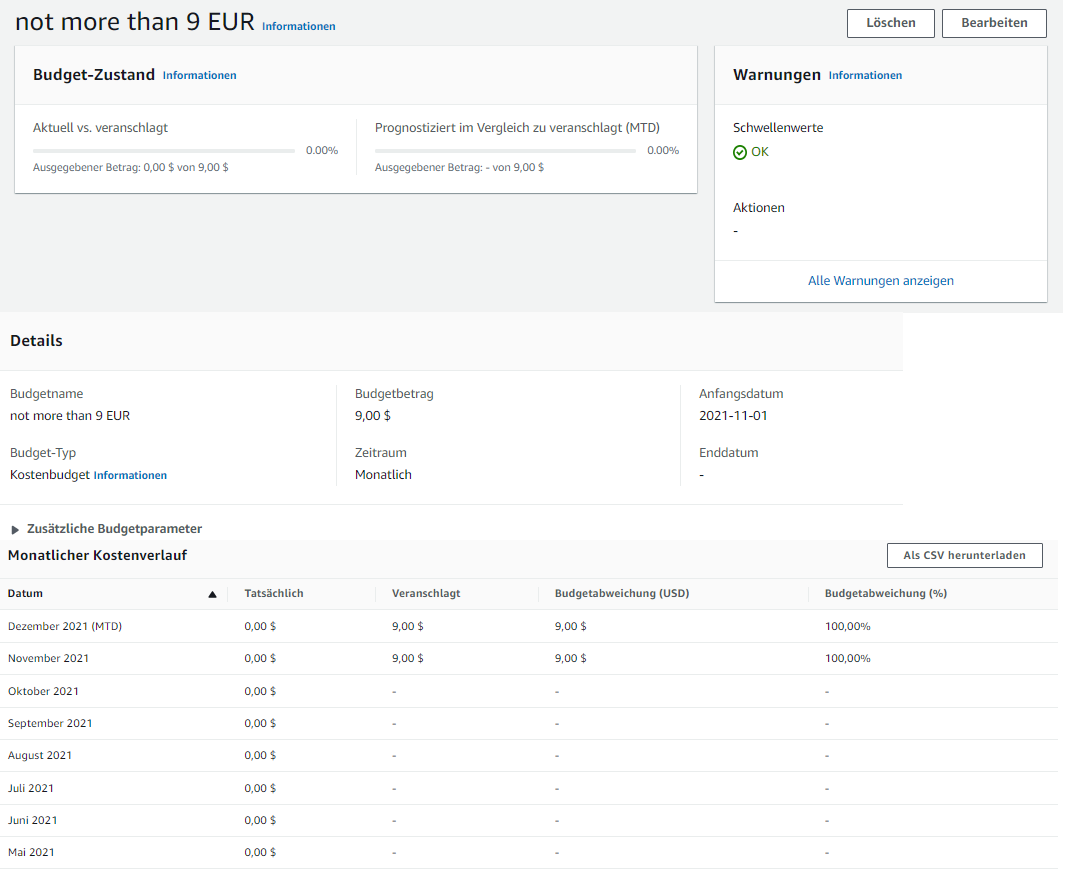
\includegraphics[scale=0.5]{sources/BudgetAlarm}
    \caption[Budgetalarm]{}
    \label{fig:CloudWatchDashboardTest} 
    Eigene Darstellung von Test AWS-Konto.
  \end{figure}

  \subsection{Screenshot des CloudWatch-Dashboards}\label{sec_Ang_C}

\newpage

% Erklärung über die selbständige Abfassung der Arbeit  
\pagestyle{empty}
\section*{Erklärung über die selbständige\\Abfassung der Arbeit} % \section*{...}: das *-Symbol erlaubt, dass dieser
% Gliederungspunkt nicht ins Inhaltsverzeichnis aufgenommen wird
\addcontentsline{toc}{section}{Erklärung über die selbständige Abfassung der Arbeit}
Ich versichere, die von mir vorgelegte Arbeit selbständig verfasst zu haben.
Alle Stellen, die wörtlich oder sinngemäß aus veröffentlichten oder nicht veröffentlichten Arbeiten anderer entnommen sind,
habe ich als entnommen kenntlich gemacht.\\
Sämtliche Quellen und Hilfsmittel, die ich für die Arbeit benutzt habe, sind
angegeben. Die Arbeit hat mit gleichem Inhalt bzw. in wesentlichen Teilen noch keiner anderen Prüfungsbehörde vorgelegen.\\\\
\begin{tabular}{cp{7cm}}
                                    &             \\
                                    &             \\ \hline
  \small (Ort, Datum, Unterschrift) & \normalsize \\
\end{tabular}

%<MERKKASTEN> (für die eigene Verwendung bitte entfernen
\vspace{1cm}
\begin{tcolorbox}[title={Hinweise zur obigen \textit{Erklärung}}]
  \begin{itemize}
    \item Bitte verwenden Sie nur die Erklärung, die Ihnen Ihr \textbf{Prüfungsservice} vorgibt. Ansonsten könnte es passieren, dass Ihre Abschlussarbeit nicht angenommen wird. Fragen Sie im Zweifelsfalle bei Ihrem Prüfungsservice nach.
    \item Sie müssen \textbf{alle abzugebende Exemplare} Ihrer Abschlussarbeit unterzeichnen. Sonst wird die Abschlussarbeit nicht akzeptiert.
    \item Ein \textbf{Verstoß} gegen die unterzeichnete \textit{Erklärung} kann u.\,a. die Aberkennung Ihres akademischen Titels zur Folge haben.
  \end{itemize}
\end{tcolorbox}
%</MERKKASTEN>   

\newpage
% Unbeschriftetes Abschlussblatt (Leere Seite)
\thispagestyle{empty}
\input{leereSeite}

\end{document}

